\documentclass[letterpaper,12pt]{article}\usepackage[]{graphicx}\usepackage[]{color}
%% maxwidth is the original width if it is less than linewidth
%% otherwise use linewidth (to make sure the graphics do not exceed the margin)
\makeatletter
\def\maxwidth{ %
  \ifdim\Gin@nat@width>\linewidth
    \linewidth
  \else
    \Gin@nat@width
  \fi
}
\makeatother

\definecolor{fgcolor}{rgb}{0.345, 0.345, 0.345}
\newcommand{\hlnum}[1]{\textcolor[rgb]{0.686,0.059,0.569}{#1}}%
\newcommand{\hlstr}[1]{\textcolor[rgb]{0.192,0.494,0.8}{#1}}%
\newcommand{\hlcom}[1]{\textcolor[rgb]{0.678,0.584,0.686}{\textit{#1}}}%
\newcommand{\hlopt}[1]{\textcolor[rgb]{0,0,0}{#1}}%
\newcommand{\hlstd}[1]{\textcolor[rgb]{0.345,0.345,0.345}{#1}}%
\newcommand{\hlkwa}[1]{\textcolor[rgb]{0.161,0.373,0.58}{\textbf{#1}}}%
\newcommand{\hlkwb}[1]{\textcolor[rgb]{0.69,0.353,0.396}{#1}}%
\newcommand{\hlkwc}[1]{\textcolor[rgb]{0.333,0.667,0.333}{#1}}%
\newcommand{\hlkwd}[1]{\textcolor[rgb]{0.737,0.353,0.396}{\textbf{#1}}}%

\usepackage{framed}
\makeatletter
\newenvironment{kframe}{%
 \def\at@end@of@kframe{}%
 \ifinner\ifhmode%
  \def\at@end@of@kframe{\end{minipage}}%
  \begin{minipage}{\columnwidth}%
 \fi\fi%
 \def\FrameCommand##1{\hskip\@totalleftmargin \hskip-\fboxsep
 \colorbox{shadecolor}{##1}\hskip-\fboxsep
     % There is no \\@totalrightmargin, so:
     \hskip-\linewidth \hskip-\@totalleftmargin \hskip\columnwidth}%
 \MakeFramed {\advance\hsize-\width
   \@totalleftmargin\z@ \linewidth\hsize
   \@setminipage}}%
 {\par\unskip\endMakeFramed%
 \at@end@of@kframe}
\makeatother

\definecolor{shadecolor}{rgb}{.97, .97, .97}
\definecolor{messagecolor}{rgb}{0, 0, 0}
\definecolor{warningcolor}{rgb}{1, 0, 1}
\definecolor{errorcolor}{rgb}{1, 0, 0}
\newenvironment{knitrout}{}{} % an empty environment to be redefined in TeX

\usepackage{alltt}
\usepackage[top=1in,bottom=1in,left=1in,right=1in]{geometry}
\usepackage{setspace}
\usepackage[colorlinks=true,urlcolor=blue,citecolor=blue,linkcolor=blue]{hyperref}
\usepackage{indentfirst}
\usepackage{multirow}
\usepackage{booktabs}
\usepackage[final]{animate}
\usepackage{graphicx}
\usepackage{verbatim}
\usepackage{rotating}
\usepackage{tabularx}
\usepackage{array}
\usepackage{subfig} 
\usepackage[noae]{Sweave}
\usepackage{cleveref}
\usepackage[figureposition=bottom]{caption}
\usepackage{paralist}
\usepackage{acronym}
\usepackage{outlines}
\usepackage{pdflscape}

% knitr options


% housekeeping


\linespread{1}
\IfFileExists{upquote.sty}{\usepackage{upquote}}{}
\begin{document}
\title{Analysis of 16S microbial sequencing data from a Southern Califoria WWTP discharge field}
\maketitle

Two datasets were used:

\begin{itemize}
\item abundance by site, separated by taxonomic level
\item environmental data by site, grouped by categories of PAH, environmental, contaminants, or metals
\end{itemize}

\begin{knitrout}
\definecolor{shadecolor}{rgb}{0.969, 0.969, 0.969}\color{fgcolor}\begin{kframe}
\begin{alltt}
\hlkwd{load}\hlstd{(}\hlkwc{file} \hlstd{=} \hlstr{'data/abudat.RData'}\hlstd{)}
\hlkwd{lapply}\hlstd{(abudat, head)}
\end{alltt}
\begin{verbatim}
## $DOMAIN
##    domain site wwtp cont abund
## 1 Archaea  CA1 LAco  int    39
## 2 Archaea CA10 ORco  int    19
## 3 Archaea CA11 SDci  int    23
## 4 Archaea CA12 ORco  clo    24
## 5 Archaea CA13 LAci  int    17
## 6 Archaea CA14 LAci  far    18
## 
## $PHYLUM
##          phylum site wwtp cont abund   domain
## 1 Acidobacteria  CA1 LAco  int    24 Bacteria
## 2 Acidobacteria CA10 ORco  int    24 Bacteria
## 3 Acidobacteria CA11 SDci  int    19 Bacteria
## 4 Acidobacteria CA12 ORco  clo    20 Bacteria
## 5 Acidobacteria CA13 LAci  int     8 Bacteria
## 6 Acidobacteria CA14 LAci  far    18 Bacteria
## 
## $CLASS
##           class site wwtp cont abund phylum domain
## 1 Acidobacteria  CA1 LAco  int     1   <NA>   <NA>
## 2 Acidobacteria CA10 ORco  int     8   <NA>   <NA>
## 3 Acidobacteria CA11 SDci  int     1   <NA>   <NA>
## 4 Acidobacteria CA12 ORco  clo     4   <NA>   <NA>
## 5 Acidobacteria CA14 LAci  far     3   <NA>   <NA>
## 6 Acidobacteria  CA2 LAco  clo     1   <NA>   <NA>
## 
## $ORDER
##               order site wwtp cont abund      class      phylum   domain
## 1 Acholeplasmatales  CA1 LAco  int    18 Mollicutes Tenericutes Bacteria
## 2 Acholeplasmatales CA10 ORco  int    21 Mollicutes Tenericutes Bacteria
## 3 Acholeplasmatales CA11 SDci  int     8 Mollicutes Tenericutes Bacteria
## 4 Acholeplasmatales CA12 ORco  clo     4 Mollicutes Tenericutes Bacteria
## 5 Acholeplasmatales CA13 LAci  int     4 Mollicutes Tenericutes Bacteria
## 6 Acholeplasmatales CA14 LAci  far     5 Mollicutes Tenericutes Bacteria
## 
## $FAMILY
##             family site wwtp cont abund            order
## 1 Acetobacteraceae  CA1 LAco  int     5 Rhodospirillales
## 2 Acetobacteraceae CA10 ORco  int     2 Rhodospirillales
## 3 Acetobacteraceae CA11 SDci  int     3 Rhodospirillales
## 4 Acetobacteraceae CA12 ORco  clo     4 Rhodospirillales
## 5 Acetobacteraceae CA13 LAci  int     1 Rhodospirillales
## 6 Acetobacteraceae CA14 LAci  far     2 Rhodospirillales
##                 class         phylum   domain
## 1 Alphaproteobacteria Proteobacteria Bacteria
## 2 Alphaproteobacteria Proteobacteria Bacteria
## 3 Alphaproteobacteria Proteobacteria Bacteria
## 4 Alphaproteobacteria Proteobacteria Bacteria
## 5 Alphaproteobacteria Proteobacteria Bacteria
## 6 Alphaproteobacteria Proteobacteria Bacteria
## 
## $GENUS
##           genus site wwtp cont abund           family            order
## 1 Acaryochloris CA12 ORco  clo     1             <NA>             <NA>
## 2 Acaryochloris CA14 LAci  far     1             <NA>             <NA>
## 3 Acaryochloris  CA4 LAco  far     1             <NA>             <NA>
## 4 Acaryochloris  CA8 SDci  far     3             <NA>             <NA>
## 5 Acaryochloris  CA9 SDci  int     1             <NA>             <NA>
## 6   Acetobacter  CA1 LAco  int     4 Acetobacteraceae Rhodospirillales
##                 class         phylum   domain
## 1                <NA>  Cyanobacteria Bacteria
## 2                <NA>  Cyanobacteria Bacteria
## 3                <NA>  Cyanobacteria Bacteria
## 4                <NA>  Cyanobacteria Bacteria
## 5                <NA>  Cyanobacteria Bacteria
## 6 Alphaproteobacteria Proteobacteria Bacteria
## 
## $SPECIES
##                    species site wwtp cont abund         genus
## 1     Acaryochloris marina CA12 ORco  clo     1 Acaryochloris
## 2     Acaryochloris marina CA14 LAci  far     1 Acaryochloris
## 3     Acaryochloris marina  CA4 LAco  far     1 Acaryochloris
## 4     Acaryochloris marina  CA8 SDci  far     3 Acaryochloris
## 5     Acaryochloris marina  CA9 SDci  int     1 Acaryochloris
## 6 Acetobacter pasteurianus  CA1 LAco  int     4   Acetobacter
##             family            order               class         phylum
## 1             <NA>             <NA>                <NA>  Cyanobacteria
## 2             <NA>             <NA>                <NA>  Cyanobacteria
## 3             <NA>             <NA>                <NA>  Cyanobacteria
## 4             <NA>             <NA>                <NA>  Cyanobacteria
## 5             <NA>             <NA>                <NA>  Cyanobacteria
## 6 Acetobacteraceae Rhodospirillales Alphaproteobacteria Proteobacteria
##     domain
## 1 Bacteria
## 2 Bacteria
## 3 Bacteria
## 4 Bacteria
## 5 Bacteria
## 6 Bacteria
\end{verbatim}
\begin{alltt}
\hlkwd{load}\hlstd{(}\hlkwc{file} \hlstd{=} \hlstr{'data/envdat.RData'}\hlstd{)}
\hlkwd{head}\hlstd{(envdat)}
\end{alltt}
\begin{verbatim}
## $con
##    site wwtp cont Acenaphthylene Anthracene Benzo.GHI.Perylene
## 1   CA1 LAco  int            0.0          0                0.0
## 2  CA10 ORco  int            0.0          0                2.2
## 3  CA11 SDci  int            0.0          0                0.0
## 4  CA12 ORco  clo            0.0          0                0.8
## 5   CA2 LAco  clo           73.5        172              324.0
## 6   CA3 LAco  int            0.0          0               70.0
## 7   CA4 LAco  far            0.0          0                0.0
## 8   CA5 ORco  far            0.0          0                0.0
## 9   CA7 SDci  clo            0.0          0                0.0
## 10  CA8 SDci  far            0.0          0               44.9
## 11  CA9 SDci  int            0.0          0                0.0
##    Benzo.K.Fluoranthene BenzoA.Anthracene BenzoA.Pyrene Chrysene
## 1                   0.0               0.0           0.0      0.0
## 2                   1.0               2.2           2.1      1.6
## 3                   0.0               0.0           0.0      0.0
## 4                   0.6               1.6           1.2      1.0
## 5                 292.0             525.0         609.0    536.0
## 6                   0.0               0.0          85.7     47.8
## 7                   0.0               0.0           0.0      0.0
## 8                   0.0               2.4           3.0      1.4
## 9                   0.0               0.0           0.0      0.0
## 10                  0.0               0.0           0.0      0.0
## 11                  0.0               0.0           0.0      0.0
##    Dibenzo.AH.Anthracene Fluorene Indeno.1.2.3.CD.Pyrene Phenanthrene
## 1                    0.0        0                    0.0          0.0
## 2                    0.0        0                    1.6          3.1
## 3                    0.0        0                    0.0          0.0
## 4                    0.0        0                    0.7          1.8
## 5                  133.0      102                  294.0        431.0
## 6                    0.0        0                    0.0          0.0
## 7                    0.0        0                    0.0          0.0
## 8                    0.0        0                    0.0          0.0
## 9                    0.0        0                    0.0          0.0
## 10                  31.3        0                   34.7          0.0
## 11                   0.0        0                    0.0          0.0
##    Pyrene Total.Detectable.DDT
## 1     0.0             1.32e+03
## 2     3.0             2.16e+00
## 3     0.0             0.00e+00
## 4     3.0             4.05e+00
## 5   864.0             1.22e+05
## 6    74.2             2.70e+03
## 7     0.0             5.91e+02
## 8     3.0             5.39e+00
## 9     0.0             0.00e+00
## 10    0.0             3.90e+02
## 11    0.0             2.50e+02
## 
## $env
##    site wwtp cont Benthic.Index.BRI.score  DEPTH.M latitude longitude
## 1   CA1 LAco  int                20.00000 61.00000 33.73000 -118.4030
## 2  CA10 ORco  int                17.69702 95.00101 32.77655 -117.4185
## 3  CA11 SDci  int                18.00000 98.00000 32.68267 -117.3278
## 4  CA12 ORco  clo                17.76361 92.81164 32.83902 -117.4814
## 5   CA2 LAco  clo                30.00000 61.00000 33.69850 -118.3360
## 6   CA3 LAco  int                20.00000 61.00000 33.70780 -118.3540
## 7   CA4 LAco  far                16.00000 61.00000 33.80720 -118.4310
## 8   CA5 ORco  far                17.73000 91.36280 32.88072 -117.5234
## 9   CA7 SDci  clo                18.00000 98.00000 32.67467 -117.3257
## 10  CA8 SDci  far                11.00000 98.00000 32.73033 -117.3428
## 11  CA9 SDci  int                24.00000 98.00000 32.66567 -117.3248
##    Total.Organic.Carbon Total.Solids
## 1                 1.300     51.50000
## 2                 0.288     69.80281
## 3                 0.568     70.60000
## 4                 0.480     68.79504
## 5                 5.600     47.60000
## 6                 1.900     53.10000
## 7                 0.940     58.50000
## 8                 0.333     68.17407
## 9                 0.543     71.50000
## 10                0.563     68.75000
## 11                0.428     72.90000
## 
## $met
##    site wwtp cont Arsenic Cadmium Copper   Lead Mercury Nickel Silver
## 1   CA1 LAco  int   10.40   1.900  38.70  23.60  0.2200  24.20  0.820
## 2  CA10 ORco  int    2.60   0.368  10.10   5.06  0.0208   7.93  0.210
## 3  CA11 SDci  int    3.79   0.174   6.09   4.98  0.0250   7.04  0.000
## 4  CA12 ORco  clo    3.44   0.663  11.90   4.41  0.0425   7.89  0.295
## 5   CA2 LAco  clo   20.40  10.700 342.00 138.00  0.9600  41.60  4.390
## 6   CA3 LAco  int   11.20   3.100  68.90  35.40  0.4100  25.20  1.640
## 7   CA4 LAco  far    6.08   0.780  18.90  14.90  0.1400  17.60  0.560
## 8   CA5 ORco  far    3.53   0.203  10.00   5.97  0.0187  11.00  0.204
## 9   CA7 SDci  clo    4.23   0.185   7.52   5.69  0.0240   7.23  0.000
## 10  CA8 SDci  far    4.16   0.143   6.30   5.14  0.0320   7.01  0.000
## 11  CA9 SDci  int    4.37   0.171   2.24   3.18  0.0190   5.20  0.000
##    Total.Chromium  Zinc
## 1            85.1 115.0
## 2            17.8  39.9
## 3            13.7  22.7
## 4            18.5  49.1
## 5           356.0 669.0
## 6           123.0 160.0
## 7            56.5  56.2
## 8            21.4  45.6
## 9            15.5  27.2
## 10           13.1  22.1
## 11           10.0  17.6
\end{verbatim}
\end{kframe}
\end{knitrout}

The analysis was conducted in two stages: 1) characterization of community structure and 2) constrained analyses to evaluate relationships between environmental characteristics and community structure.  The first set of analyses included basic statistical methods (e.g., abundance barplots, diversity measures, etc.) and more specific community-level analyses such as cluster analysis and ordination to characterize site-level variation.  Indirect gradient analyses were also used to describe groupings in the data, e.g., visual separation of ordination plots by factor groupings.  The second set of analyses  used direct gradient analyses to identify relationships between environmental data and community structure.  Specifically, redundancy analysis was used to group sites by taxonomic units while constraining the relationships by environmental parameters.  All analyses considered the effects of taxonomic resolution and the relative influence on conclusions with separate analyses by domain (archaea and bacteria).

\section{Community structure}
Basic barplots of abundance are shown first by identifying the top 10 most abundant species across all locations.  The remaining plots retain these species to visualize potential variation by municipal location (e.g., city of LA, LA county, etc.), site treatment designations from metadata (i.e., location relative to a WWTP outflow), and actual site designations.  These plots are produced as a visual comparison that may potentially explain results that follow.  The remaining figures attempt to identify community structure through taxonomic abundance alone by evaluating the data at different taxonomic resolutions (phylum, class, etc.) and different spatial groupings (individual sites, distance categories by outflow, etc.).  Clustering and ordination are used to reduce dimensionality of the data based on the underlying structure of the taxonomic information.  The objective of both analyses is to identify natural groupings in the data, where groupings could be defined by the different spatial categories and may also vary by taxonomic resolution.  Direct analyses related to environmental parameters could help explain this variation further.  Finally, the tables of alpha and beta diversity explain diversity at each location (alpha) and diversity across a gradient (beta, or diversity between spatial units).  Diversity can be measured several ways and additional estimates should be considered in further analyses.    
\begin{knitrout}
\definecolor{shadecolor}{rgb}{0.969, 0.969, 0.969}\color{fgcolor}\begin{figure}[!ht]

{\centering 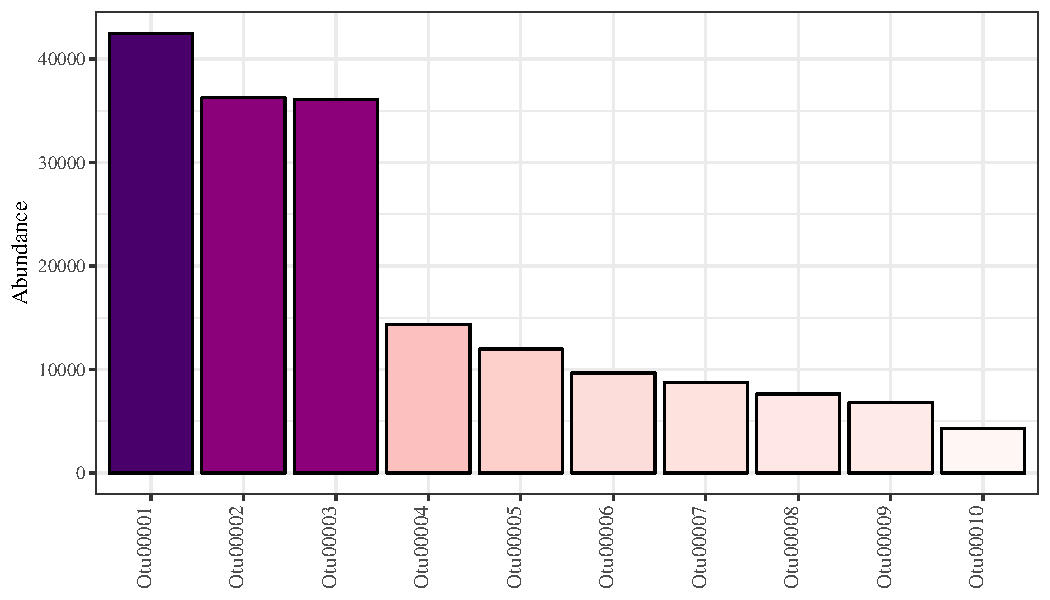
\includegraphics[width=0.8\textwidth]{figs/abundall-1} 

}

\caption[Top fifty most abundant species across all study sites]{Top fifty most abundant species across all study sites.}\label{fig:abundall}
\end{figure}


\end{knitrout}

\begin{knitrout}
\definecolor{shadecolor}{rgb}{0.969, 0.969, 0.969}\color{fgcolor}\begin{figure}[!ht]

{\centering 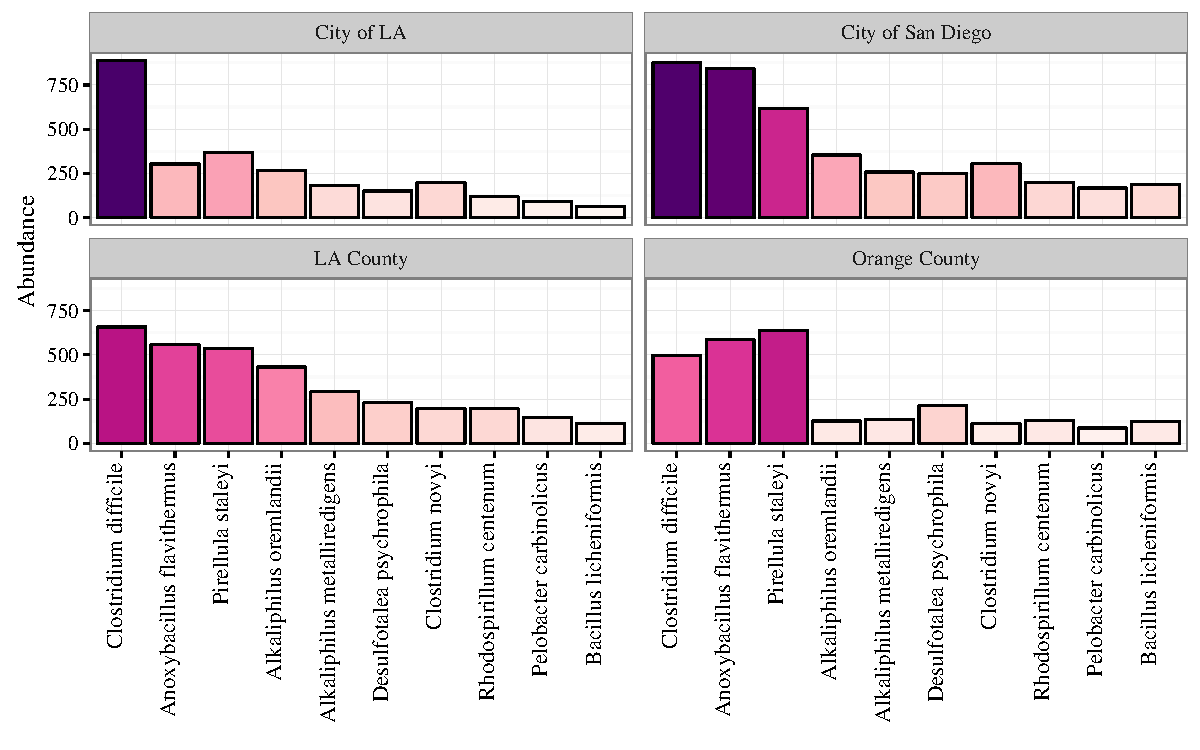
\includegraphics[width=0.8\textwidth]{figs/abundmuni-1} 

}

\caption{Species abundances by municipal locations using the top fifty most abundant across all study sites in \cref{fig:abundall}.}\label{fig:abundmuni}
\end{figure}


\end{knitrout}
\clearpage

\begin{knitrout}
\definecolor{shadecolor}{rgb}{0.969, 0.969, 0.969}\color{fgcolor}\begin{figure}[!ht]

{\centering 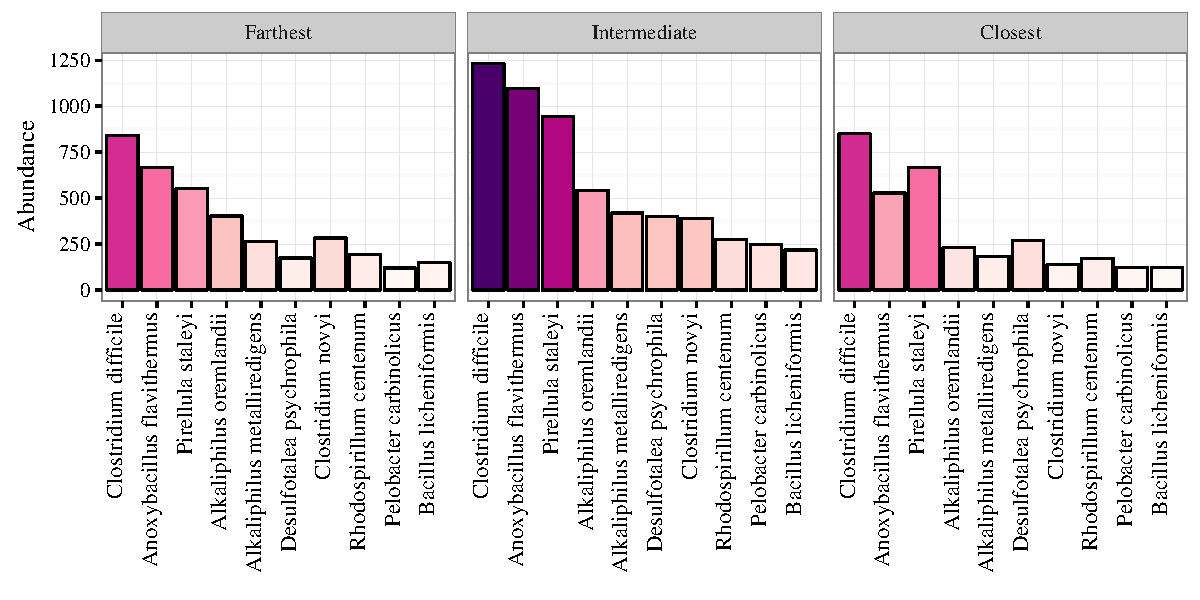
\includegraphics[width=0.8\textwidth]{figs/abundcont-1} 

}

\caption{Species abundances by distance from pipe for the top fifty most abundant across all study sites in \cref{fig:abundall}.  Treatments are based on relative distances from an outflow pipe (farthest, intermediate, closest) for each municipality.}\label{fig:abundcont}
\end{figure}


\end{knitrout}
\clearpage

\begin{landscape}
\centering\vspace*{\fill}
\begin{knitrout}
\definecolor{shadecolor}{rgb}{0.969, 0.969, 0.969}\color{fgcolor}\begin{figure}[!ht]

{\centering 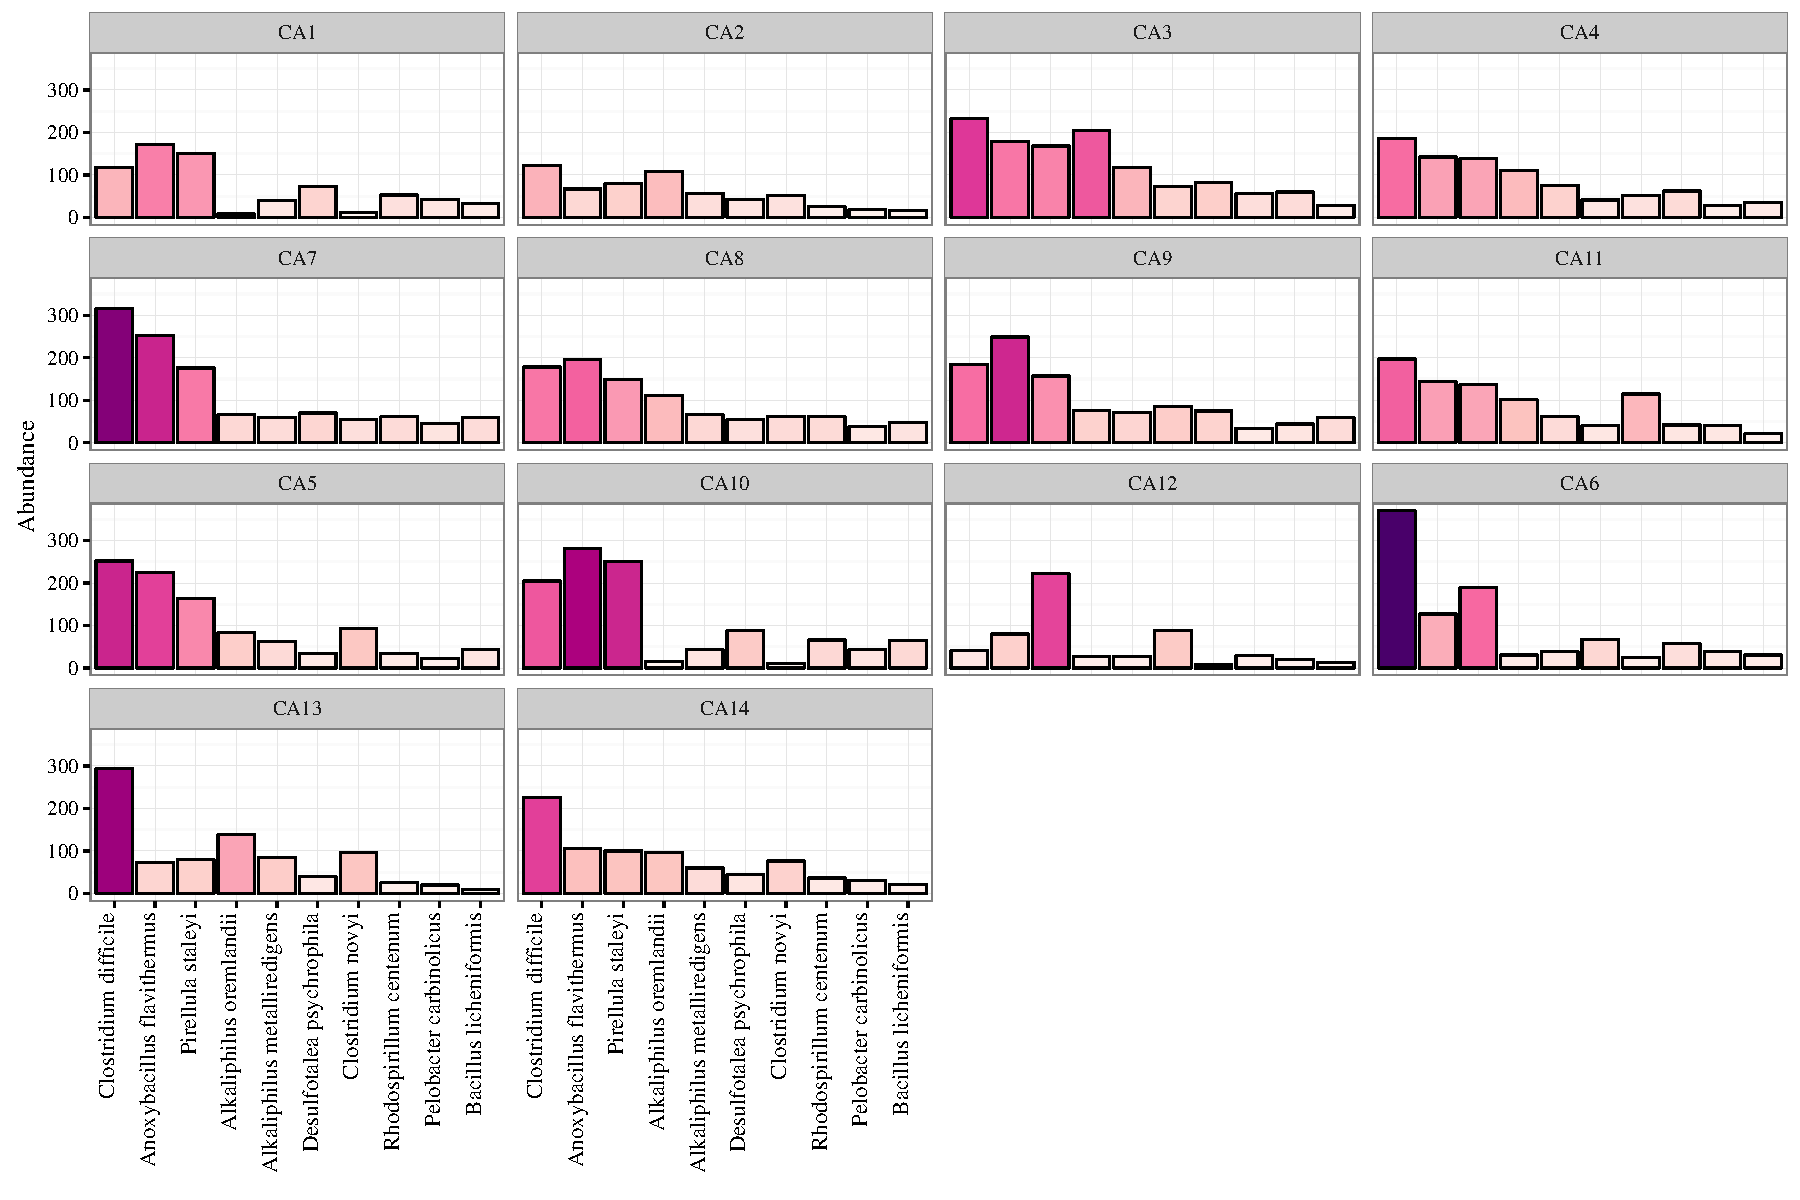
\includegraphics[width=1.1\textwidth]{figs/abundsite-1} 

}

\caption{Species abundances by sites using the top fifty most abundant across all study sites in \cref{fig:abundall}.}\label{fig:abundsite}
\end{figure}


\end{knitrout}
\end{landscape}
\clearpage

\subsection{Multivariate analyses with archaea}

\begin{knitrout}
\definecolor{shadecolor}{rgb}{0.969, 0.969, 0.969}\color{fgcolor}\begin{figure}[!ht]

{\centering 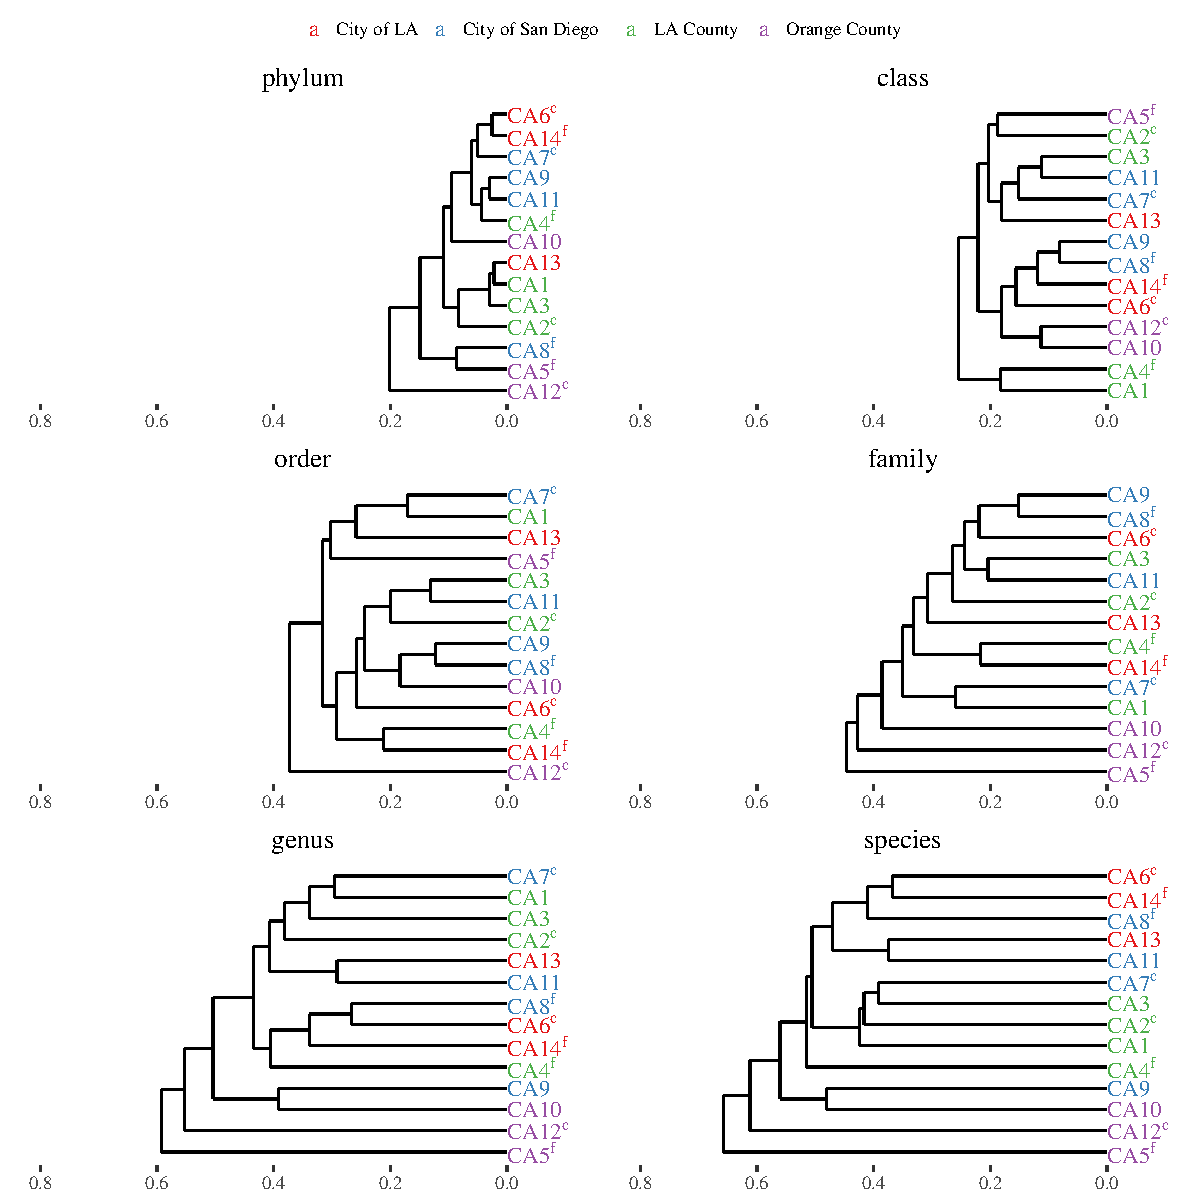
\includegraphics[width=\textwidth]{figs/clust1_arch-1} 

}

\caption[Site clusters of archaea by taxonomic resolution]{Site clusters of archaea by taxonomic resolution.  Colors indicate municipality and superscripts indicate distance categories from an outflow pipe at each site (`f' is farthest, `c' is closest, none is intermediate).  Clustering was based on a Bray-Curtis dissimilarity matrix of abundance data and sorting using the unweighted pair group method.}\label{fig:clust1_arch}
\end{figure}


\end{knitrout}

\begin{knitrout}
\definecolor{shadecolor}{rgb}{0.969, 0.969, 0.969}\color{fgcolor}\begin{figure}[!ht]

{\centering 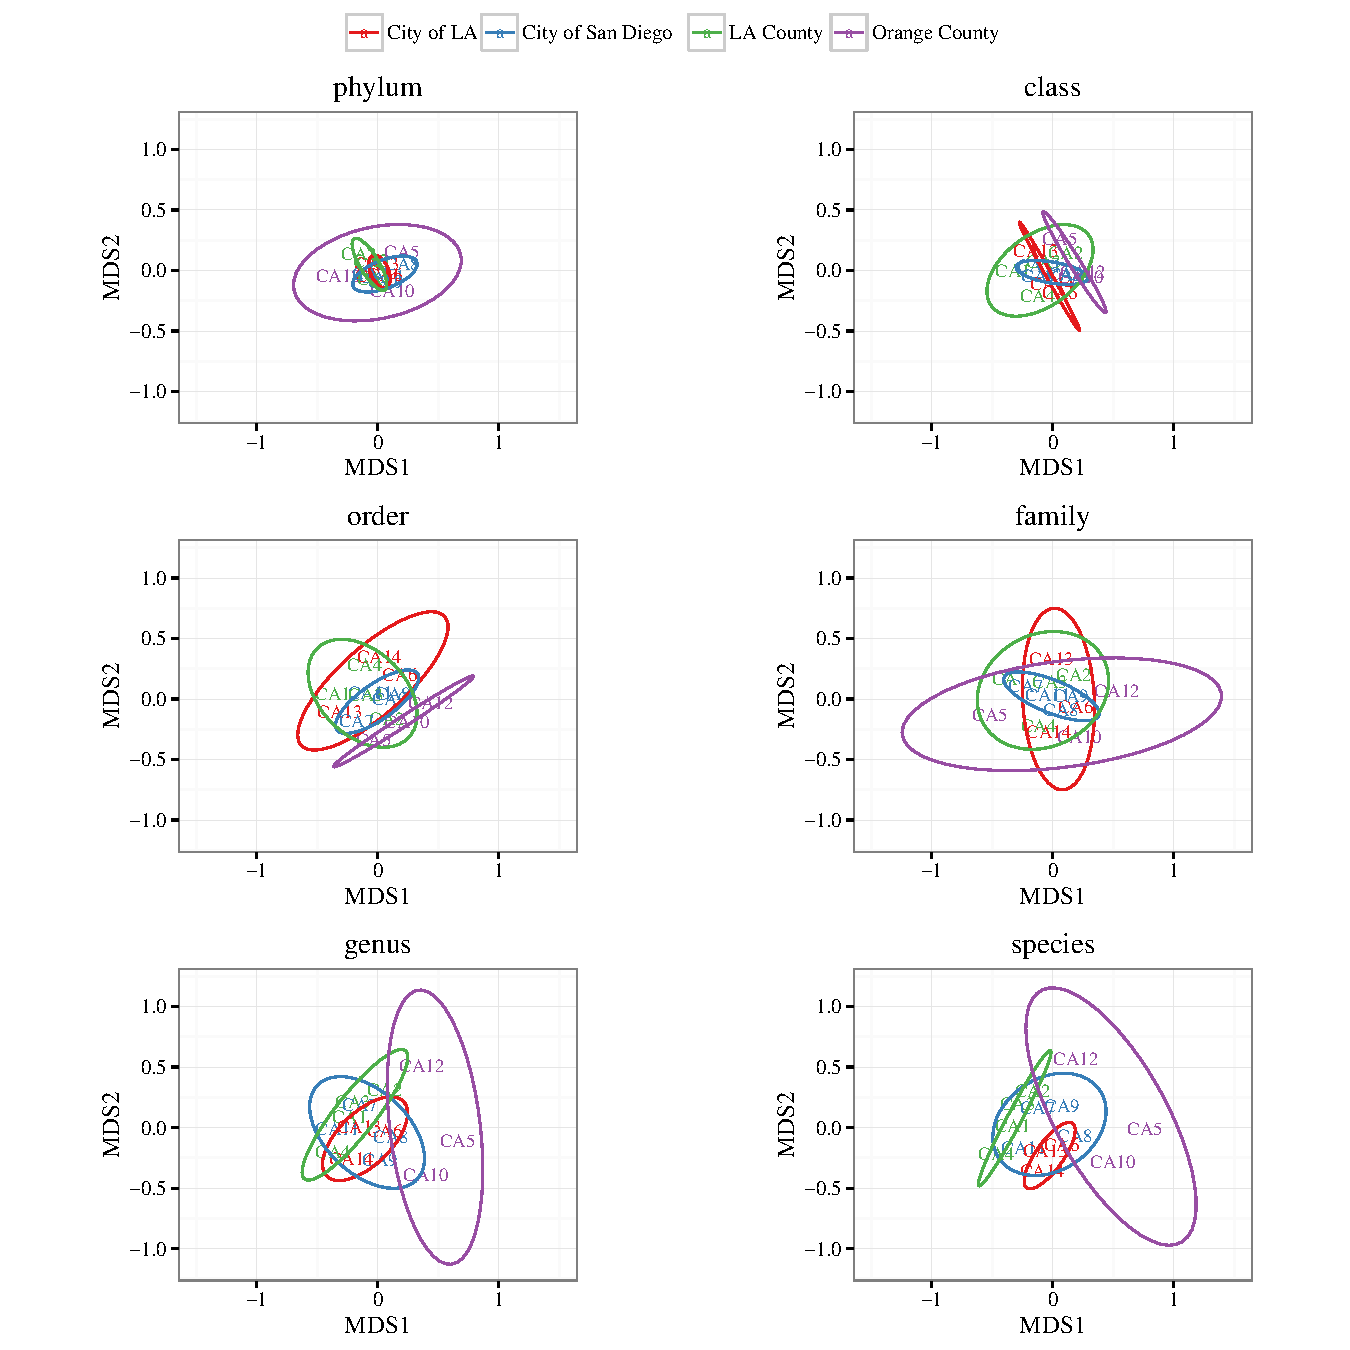
\includegraphics[width=\textwidth]{figs/ord1_arch-1} 

}

\caption{Site ordinations of archaea by taxonomic resolution.  Colors indicate municipality with ellipses showing 95\% bivariate confidence intervals.  Ordinations were created using Nonmetric Multidimensional scaling with several random starts to find a stable solution of the configuration.  A Bray-Curtis dissimilarity matrix was used as a measure of differences between sites. The ordination is the same as in \cref{fig:ord2_arch} but with different group categories in the plot.}\label{fig:ord1_arch}
\end{figure}


\end{knitrout}

\begin{knitrout}
\definecolor{shadecolor}{rgb}{0.969, 0.969, 0.969}\color{fgcolor}\begin{figure}[!ht]

{\centering 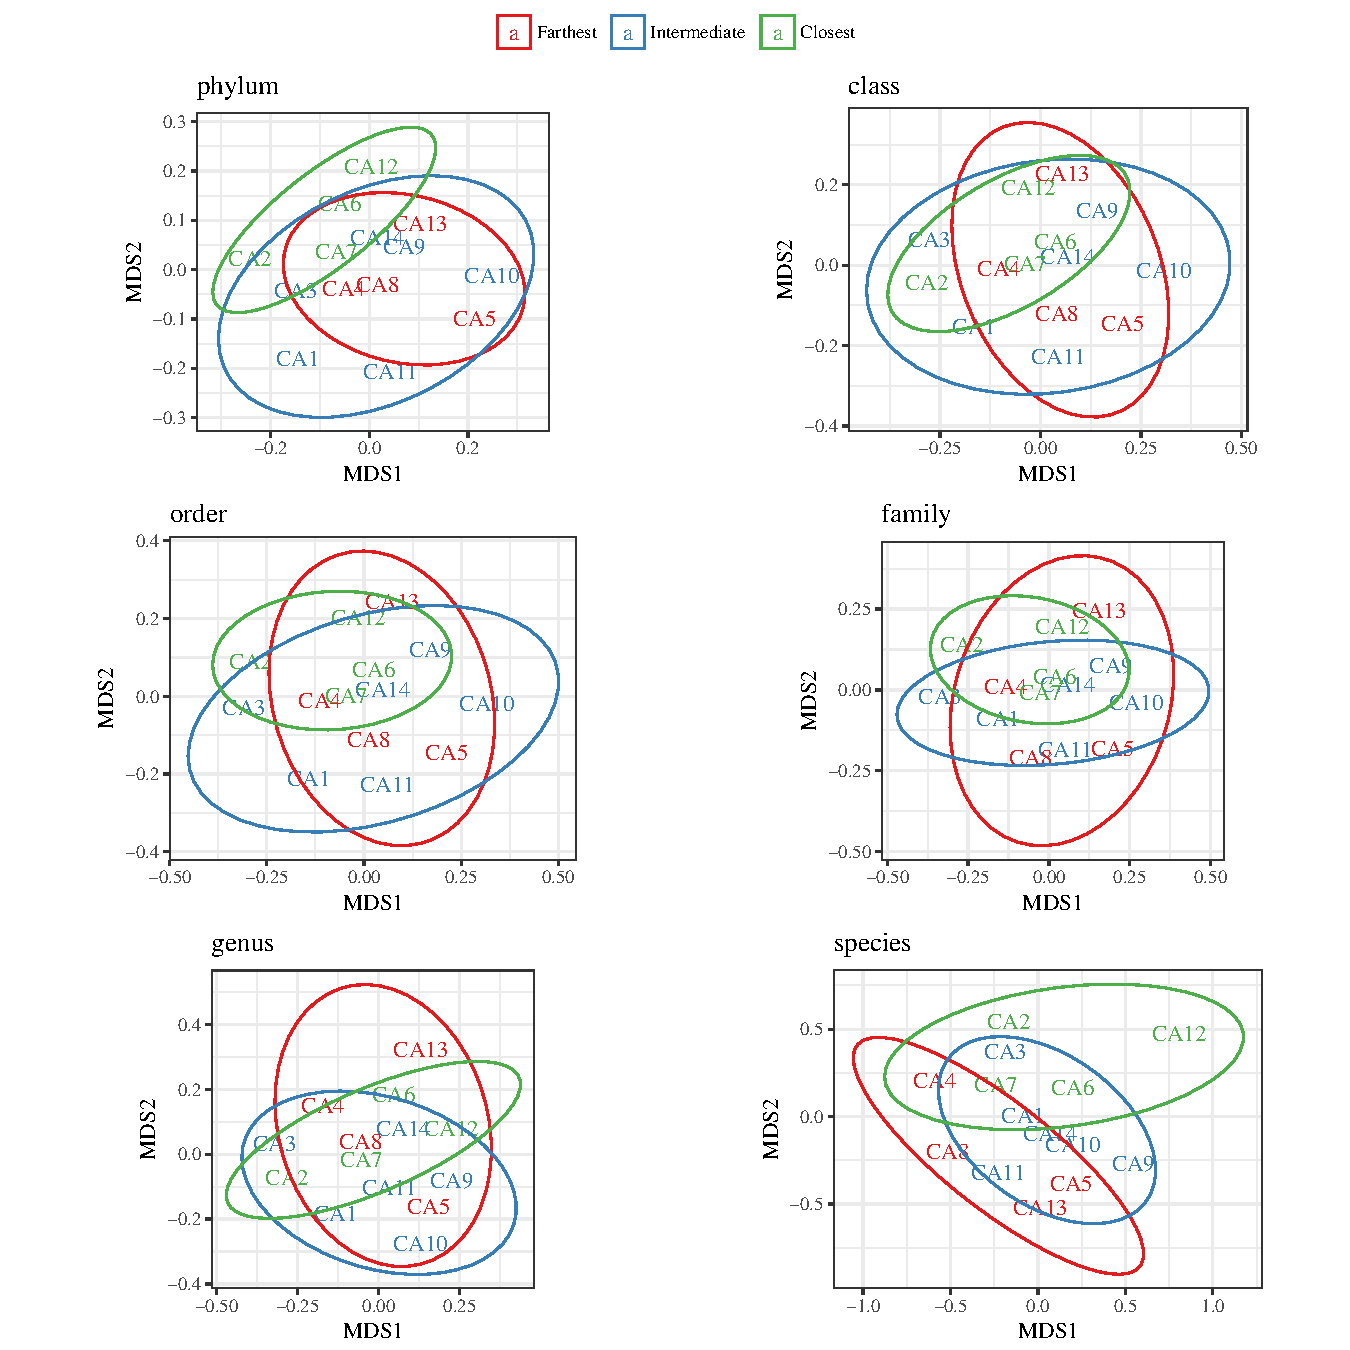
\includegraphics[width=1.05\textwidth]{figs/ord2_arch-1} 

}

\caption{Site ordinations of archaea by taxonomic resolution.  Colors indicate approximate distance from pipe with ellipses showing 95\% bivariate confidence intervals. Ordinations were created using Nonmetric Multidimensional scaling with several random starts to find a stable solution of the configuration.  A Bray-Curtis dissimilarity matrix was used as a measure of differences between sites. The ordination is the same as in \cref{fig:ord1_arch} but with different group categories in the plot.}\label{fig:ord2_arch}
\end{figure}


\end{knitrout}
\clearpage

%latex.default(taba, file = "", rowlabel = "Location grouping",     caption = cap.val, caption.loc = "top", rgroup = c("Municipality",         "Pipe location", "Site"), n.rgroup = c(4, 3, 14), rowname = rows,     label = "tab:alpha_arch")%
\begin{table}[!tbp]
\caption{Alpha diversity of archaea by municipality, distance from outflow, and sites for each taxonomic level.  Original data were taxanomic abundance aggregated by each grouping.  Alpha was was based on methods in Fisher et al. (1943) that measure diversity as a function of richness and abundance at a site.\label{tab:alpha_arch}} 
\begin{center}
\begin{tabular}{lllllll}
\hline\hline
\multicolumn{1}{l}{Location grouping}&\multicolumn{1}{c}{Phylum}&\multicolumn{1}{c}{Class}&\multicolumn{1}{c}{Order}&\multicolumn{1}{c}{Family}&\multicolumn{1}{c}{Genus}&\multicolumn{1}{c}{Species}\tabularnewline
\hline
{\bfseries Municipality}&&&&&&\tabularnewline
~~City of LA&0.92&1.75&3.83& 3.95& 6.54&10.28\tabularnewline
~~City of San Diego&0.77&1.70&3.22& 4.56&12.43&17.32\tabularnewline
~~LA County&0.70&1.78&3.28& 4.81&11.85&18.14\tabularnewline
~~Orange County&0.95&1.75&3.95& 6.49&17.90&20.82\tabularnewline
\hline
{\bfseries Pipe location}&&&&&&\tabularnewline
~~Farthest&0.82&2.28&4.06& 4.60&11.20&17.45\tabularnewline
~~Intermediate&0.71&1.83&3.28& 4.87&12.23&19.17\tabularnewline
~~Closest&0.72&1.54&3.01& 4.53&10.31&16.37\tabularnewline
\hline
{\bfseries Site}&&&&&&\tabularnewline
~~CA1&1.12&3.00&4.99& 7.67&15.68&26.56\tabularnewline
~~CA2&0.87&1.62&3.77& 4.47&11.62&16.53\tabularnewline
~~CA3&0.99&1.96&4.71& 7.22&12.12&22.29\tabularnewline
~~CA4&1.22&3.32&5.56& 5.75&14.66&20.87\tabularnewline
~~CA7&1.10&2.72&3.73& 6.61&15.42&19.33\tabularnewline
~~CA8&1.15&2.02&4.88& 5.12& 8.42&12.59\tabularnewline
~~CA9&1.13&1.74&4.50& 6.78&17.08&21.80\tabularnewline
~~CA11&1.40&3.15&8.75&10.03&18.71&29.47\tabularnewline
~~CA5&1.50&3.98&5.52& 5.52&10.03&12.67\tabularnewline
~~CA10&1.00&2.63&5.21& 5.52&24.03&24.03\tabularnewline
~~CA12&0.90&1.97&4.35& 5.44&17.12&20.98\tabularnewline
~~CA6&1.18&1.88&4.16& 4.16& 6.61&10.26\tabularnewline
~~CA13&1.65&2.97&6.97&10.49&18.17&18.17\tabularnewline
~~CA14&1.59&2.78&4.45& 4.75& 9.26&21.00\tabularnewline
\hline
\end{tabular}\end{center}

\end{table}
%latex.default(tabb, file = "", rowlabel = "Location grouping",     caption = cap.val, caption.loc = "top", rowname = rows, label = "tab:beta_arch")%
\begin{table}[!tbp]
\caption{Beta diversity of archaea between municipalities, distance categories from outflow, and sites for each taxonomic level.  Original data were taxonomic abundance aggregated by each grouping.  Beta was estimated as total species richness across all categories in each grouping, divided by mean species richness within each category, minus one.\label{tab:beta_arch}} 
\begin{center}
\begin{tabular}{lllllll}
\hline\hline
\multicolumn{1}{l}{Location grouping}&\multicolumn{1}{c}{Phylum}&\multicolumn{1}{c}{Class}&\multicolumn{1}{c}{Order}&\multicolumn{1}{c}{Family}&\multicolumn{1}{c}{Genus}&\multicolumn{1}{c}{Species}\tabularnewline
\hline
Distance from outflow&0.00&0.04&0.03&0.15&0.27&0.31\tabularnewline
Site&0.04&0.40&0.40&0.77&1.40&1.84\tabularnewline
Municipality&0.00&0.19&0.11&0.24&0.41&0.58\tabularnewline
\hline
\end{tabular}\end{center}

\end{table}


\subsection{Multivariate analyses with bacteria}

The above analyses (clustering, ordination, diversity) were repeated using only bacteria.  

\begin{knitrout}
\definecolor{shadecolor}{rgb}{0.969, 0.969, 0.969}\color{fgcolor}\begin{figure}[!ht]

{\centering 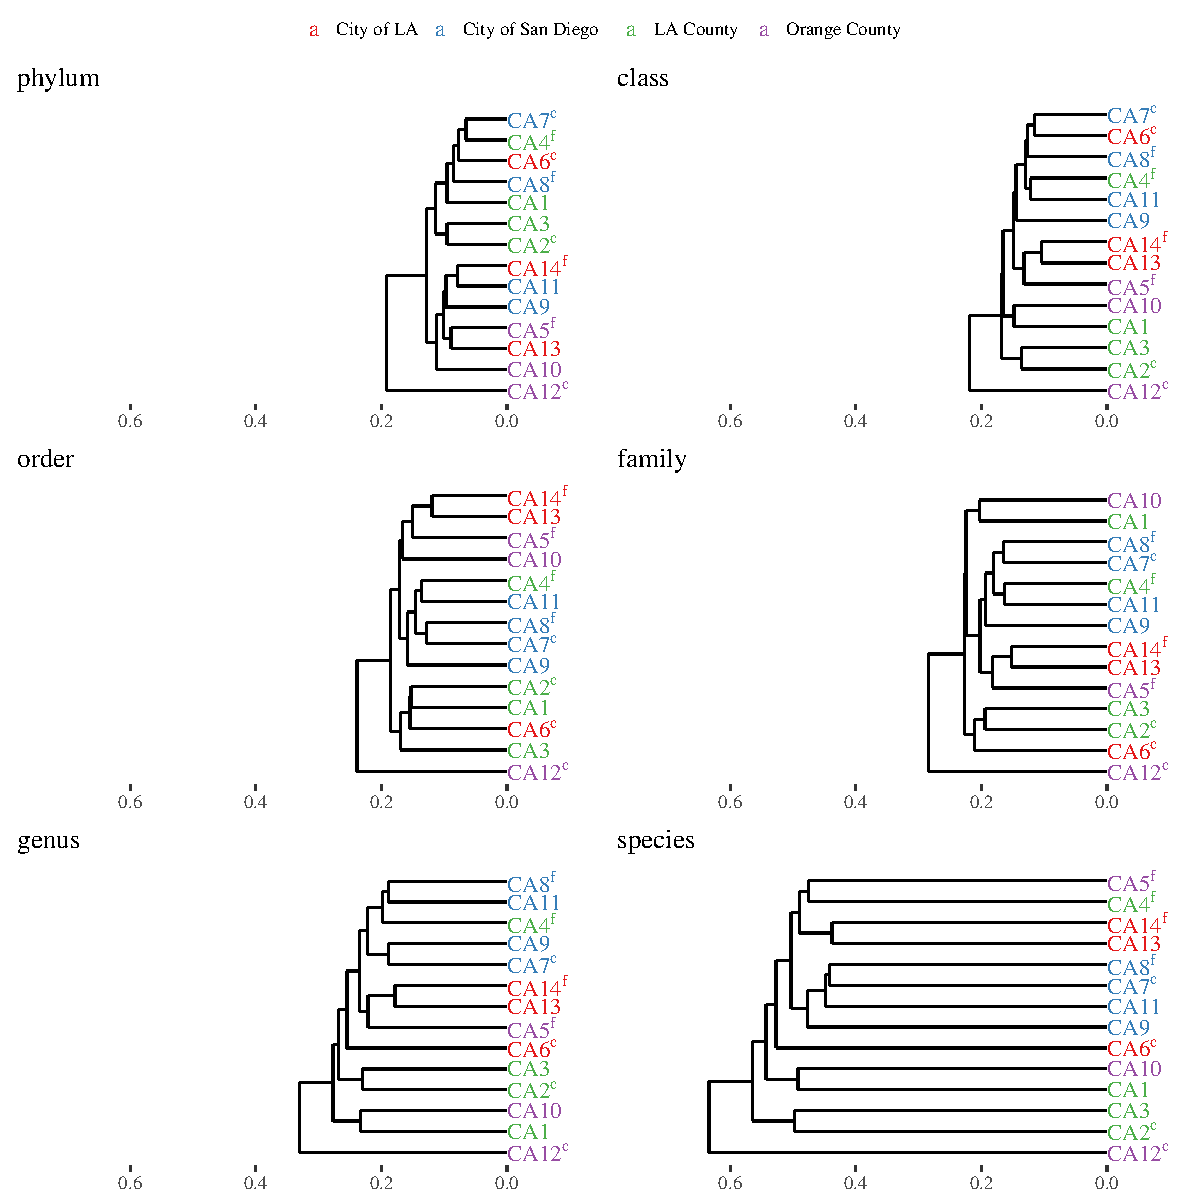
\includegraphics[width=\textwidth]{figs/clust1_bac-1} 

}

\caption[Site clusters of bacteria by taxonomic resolution]{Site clusters of bacteria by taxonomic resolution.  Colors indicate municipality and superscripts indicate distance categories from an outflow pipe at each site (`f' is farthest, `c' is closest, none is intermediate).  Clustering was based on a Bray-Curtis dissimilarity matrix of abundance data and sorting using the unweighted pair group method.}\label{fig:clust1_bac}
\end{figure}


\end{knitrout}

\begin{knitrout}
\definecolor{shadecolor}{rgb}{0.969, 0.969, 0.969}\color{fgcolor}\begin{figure}[!ht]

{\centering 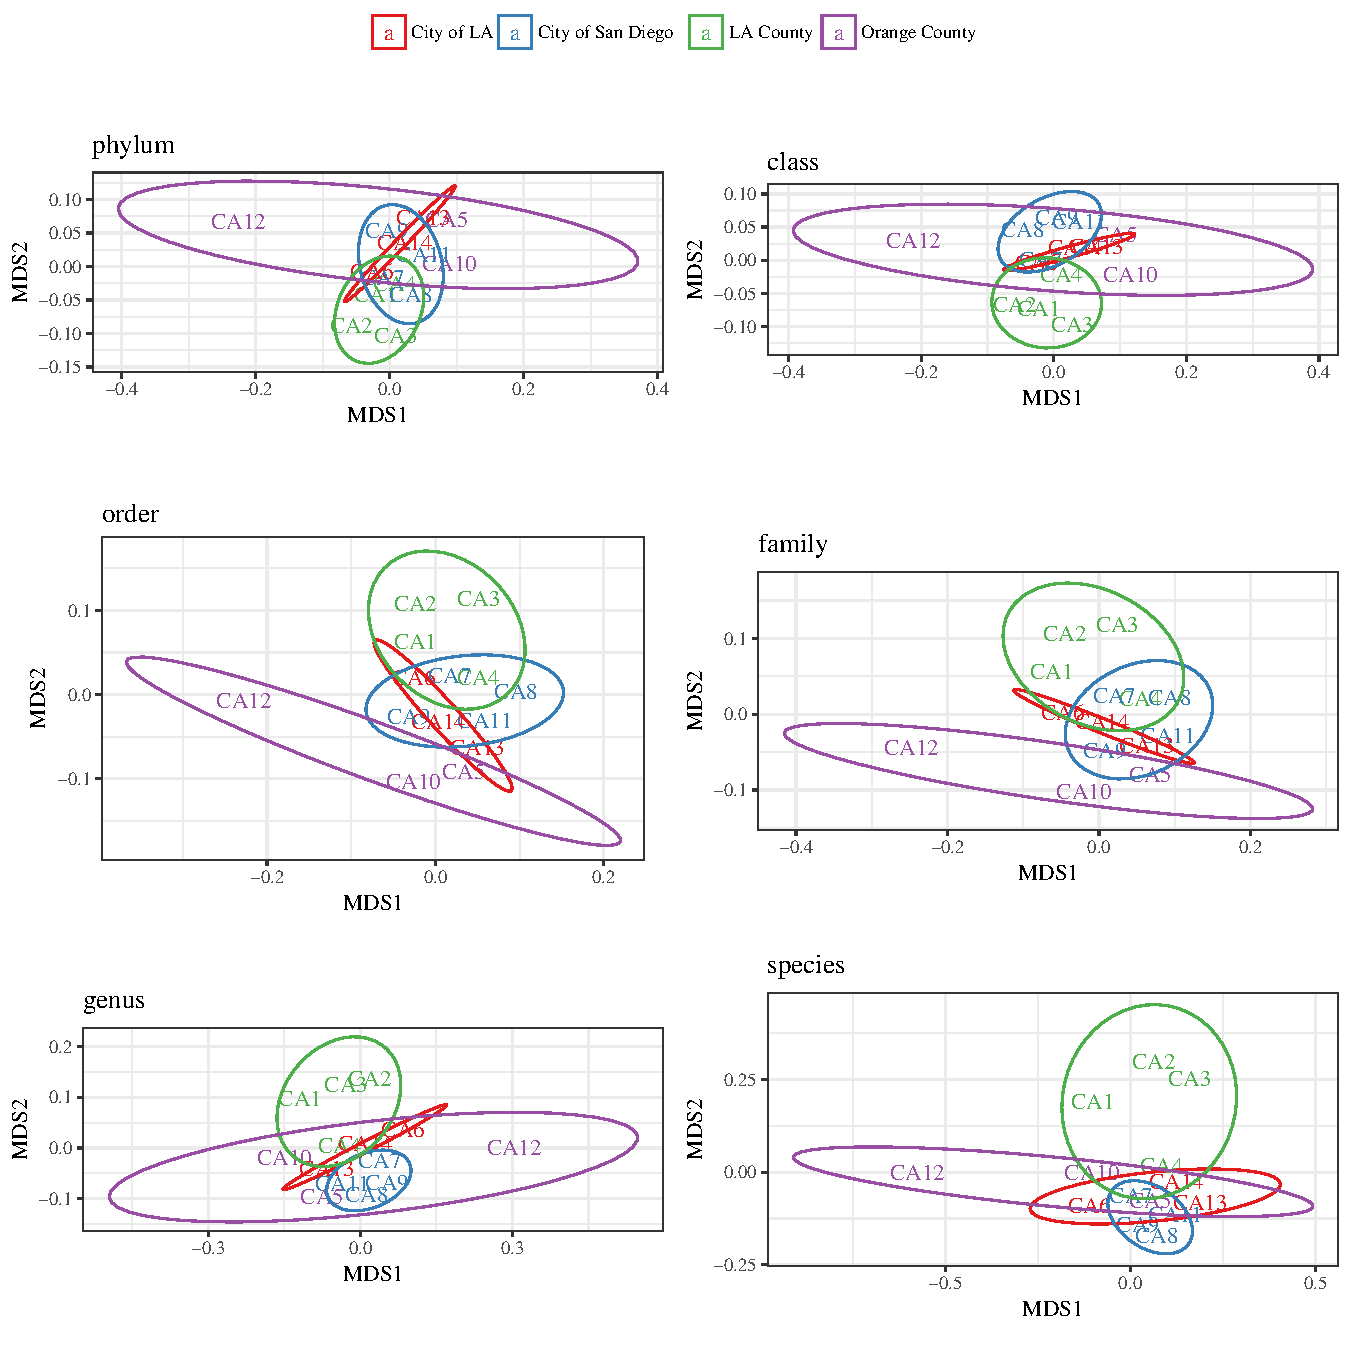
\includegraphics[width=\textwidth]{figs/ord1_bac-1} 

}

\caption{Site ordinations of bacteria by taxonomic resolution.  Colors indicate municipality with ellipses showing 95\% bivariate confidence intervals.  Ordinations were created using Nonmetric Multidimensional scaling with several random starts to find a stable solution of the configuration.  A Bray-Curtis dissimilarity matrix was used as a measure of differences between sites. The ordination is the same as in \cref{fig:ord2_bac} but with different group categories in the plot.}\label{fig:ord1_bac}
\end{figure}


\end{knitrout}

\begin{knitrout}
\definecolor{shadecolor}{rgb}{0.969, 0.969, 0.969}\color{fgcolor}\begin{figure}[!ht]

{\centering 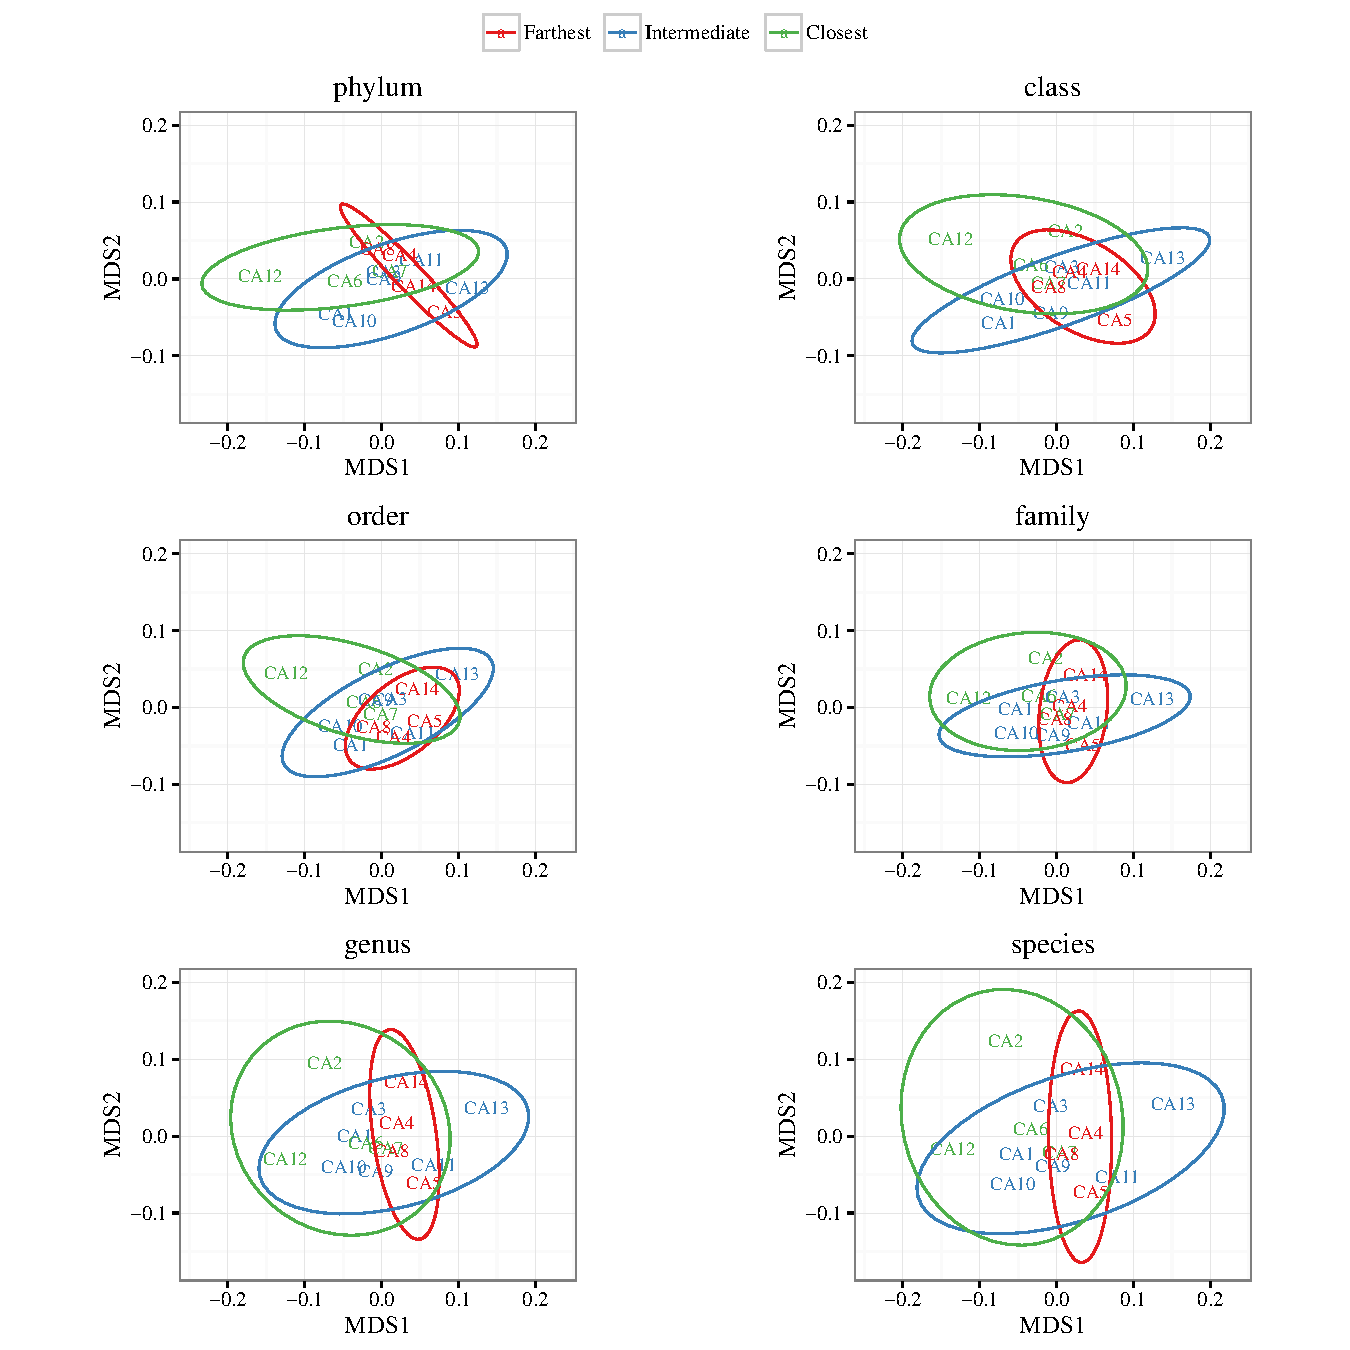
\includegraphics[width=1.05\textwidth]{figs/ord2_bac-1} 

}

\caption{Site ordinations of bacteria by taxonomic resolution.  Colors indicate approximate distance from pipe with ellipses showing 95\% bivariate confidence intervals. Ordinations were created using Nonmetric Multidimensional scaling with several random starts to find a stable solution of the configuration.  A Bray-Curtis dissimilarity matrix was used as a measure of differences between sites. The ordination is the same as in \cref{fig:ord1_bac} but with different group categories in the plot.}\label{fig:ord2_bac}
\end{figure}


\end{knitrout}
\clearpage

%latex.default(taba, file = "", rowlabel = "Location grouping",     caption = cap.val, caption.loc = "top", rgroup = c("Municipality",         "Pipe location", "Site"), n.rgroup = c(4, 3, 14), rowname = rows,     label = "tab:alpha_bac")%
\begin{table}[!tbp]
\caption{Alpha diversity of bacteria by municipality, distance from outflow, and sites for each taxonomic level.  Original data were taxanomic abundance aggregated by each grouping.  Alpha was was based on methods in Fisher et al. (1943) that measure diversity as a function of richness and abundance at a site.\label{tab:alpha_bac}} 
\begin{center}
\begin{tabular}{lllllll}
\hline\hline
\multicolumn{1}{l}{Location grouping}&\multicolumn{1}{c}{Phylum}&\multicolumn{1}{c}{Class}&\multicolumn{1}{c}{Order}&\multicolumn{1}{c}{Family}&\multicolumn{1}{c}{Genus}&\multicolumn{1}{c}{Species}\tabularnewline
\hline
{\bfseries Municipality}&&&&&&\tabularnewline
~~City of LA&2.94&2.70&12.25&27.99&63.00&112.49\tabularnewline
~~City of San Diego&2.62&2.53&11.48&25.67&58.47&107.51\tabularnewline
~~LA County&2.81&2.57&11.76&26.24&61.17&112.66\tabularnewline
~~Orange County&2.73&2.64&11.89&27.26&62.67&115.03\tabularnewline
\hline
{\bfseries Pipe location}&&&&&&\tabularnewline
~~Farthest&2.82&2.59&11.63&26.31&60.22&110.04\tabularnewline
~~Intermediate&2.63&2.41&10.99&24.37&56.34&104.76\tabularnewline
~~Closest&2.76&2.54&11.52&26.22&61.50&114.47\tabularnewline
\hline
{\bfseries Site}&&&&&&\tabularnewline
~~CA1&3.14&2.69&13.97&33.47&73.05&124.89\tabularnewline
~~CA2&3.13&3.21&15.14&33.38&71.11&120.62\tabularnewline
~~CA3&3.15&3.05&14.42&31.10&67.72&114.19\tabularnewline
~~CA4&2.98&3.04&12.84&30.60&67.92&117.63\tabularnewline
~~CA7&3.16&3.05&13.73&31.03&67.59&113.34\tabularnewline
~~CA8&3.21&3.11&13.82&30.43&68.86&119.38\tabularnewline
~~CA9&3.23&2.94&13.92&31.02&65.83&113.72\tabularnewline
~~CA11&3.38&3.08&14.27&32.33&65.75&107.74\tabularnewline
~~CA5&3.20&3.08&14.27&33.03&66.61&110.66\tabularnewline
~~CA10&2.97&3.04&13.37&29.81&64.75&116.99\tabularnewline
~~CA12&3.23&2.99&14.40&33.57&74.51&132.09\tabularnewline
~~CA6&3.17&3.09&14.00&32.52&71.31&124.14\tabularnewline
~~CA13&3.10&2.98&13.77&29.10&58.23& 97.39\tabularnewline
~~CA14&3.61&3.13&15.03&32.57&66.15&109.92\tabularnewline
\hline
\end{tabular}\end{center}

\end{table}
%latex.default(tabb, file = "", rowlabel = "Location grouping",     caption = cap.val, caption.loc = "top", rowname = rows, label = "tab:beta_bac")%
\begin{table}[!tbp]
\caption{Beta diversity of bacteria between municipalities, distance categories from outflow, and sites for each taxonomic level.  Original data were taxonomic abundance aggregated by each grouping.  Beta was estimated as total species richness across all categories in each grouping, divided by mean species richness within each category, minus one.\label{tab:beta_bac}} 
\begin{center}
\begin{tabular}{lllllll}
\hline\hline
\multicolumn{1}{l}{Location grouping}&\multicolumn{1}{c}{Phylum}&\multicolumn{1}{c}{Class}&\multicolumn{1}{c}{Order}&\multicolumn{1}{c}{Family}&\multicolumn{1}{c}{Genus}&\multicolumn{1}{c}{Species}\tabularnewline
\hline
Distance from outflow&0.00&0.00&0.01&0.01&0.05&0.12\tabularnewline
Site&0.07&0.04&0.09&0.14&0.33&0.58\tabularnewline
Municipality&0.02&0.00&0.02&0.02&0.08&0.17\tabularnewline
\hline
\end{tabular}\end{center}

\end{table}


\section{Identifying drivers of community structure}

The environmental data was grouped by categories and summarized into principal components.  This was done to reduce the dimensionality of the data given the sample sizes.  The grouping categories included contaminants, environmental, and metals.  Sites and variables with more than 50\% of the data missing were removed.  Although plots are shows, stepwise variable selection of parameters in the constrained indicated that none of the principal component axes explained any significant portion of the variation in community composition. 

\begin{knitrout}
\definecolor{shadecolor}{rgb}{0.969, 0.969, 0.969}\color{fgcolor}\begin{figure}[!ht]

{\centering 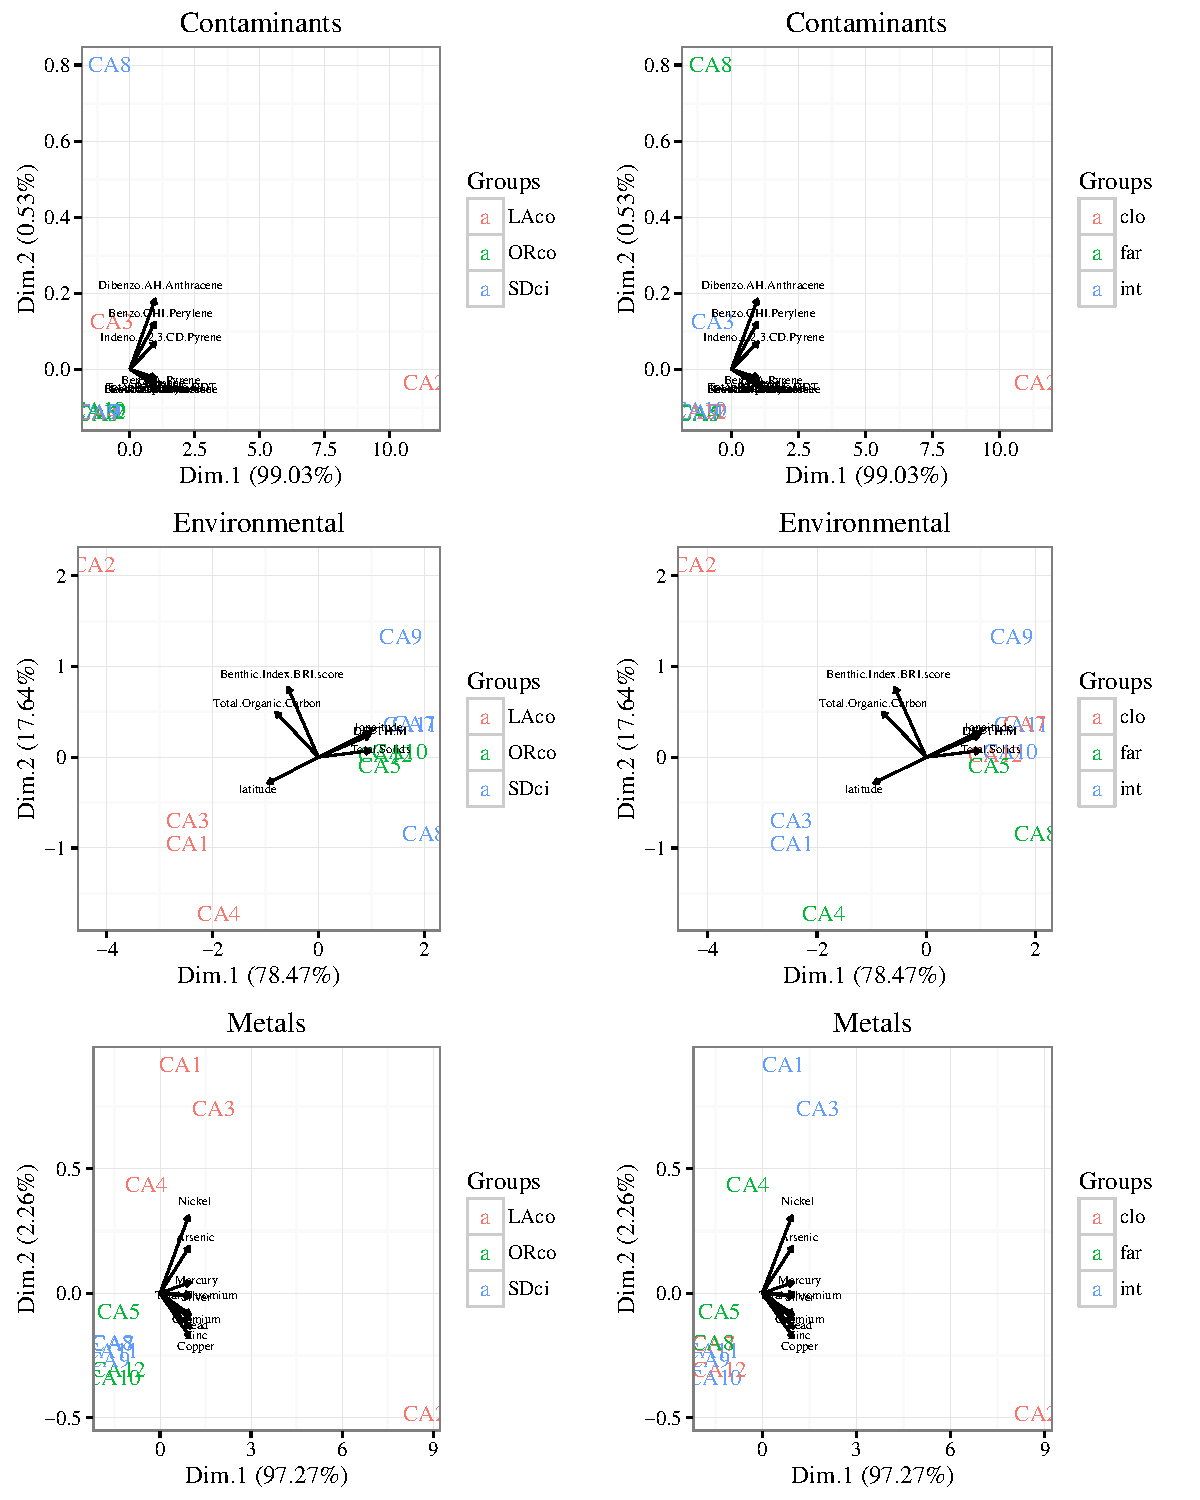
\includegraphics[width=\textwidth]{figs/unnamed-chunk-5-1} 

}

\caption[Principal component axes for contaminants, environmental, and metals, grouped by municipality and distance from pipe]{Principal component axes for contaminants, environmental, and metals, grouped by municipality and distance from pipe.}\label{fig:unnamed-chunk-5}
\end{figure}


\end{knitrout}

Constrained ordination analyses (RDA using site x species matrix and site by environmental matrix as PC scores) was used to relate archaea and bacterial communities to the environmental categories.  This was done for species and orders.
\begin{knitrout}
\definecolor{shadecolor}{rgb}{0.969, 0.969, 0.969}\color{fgcolor}\begin{figure}[!ht]

{\centering 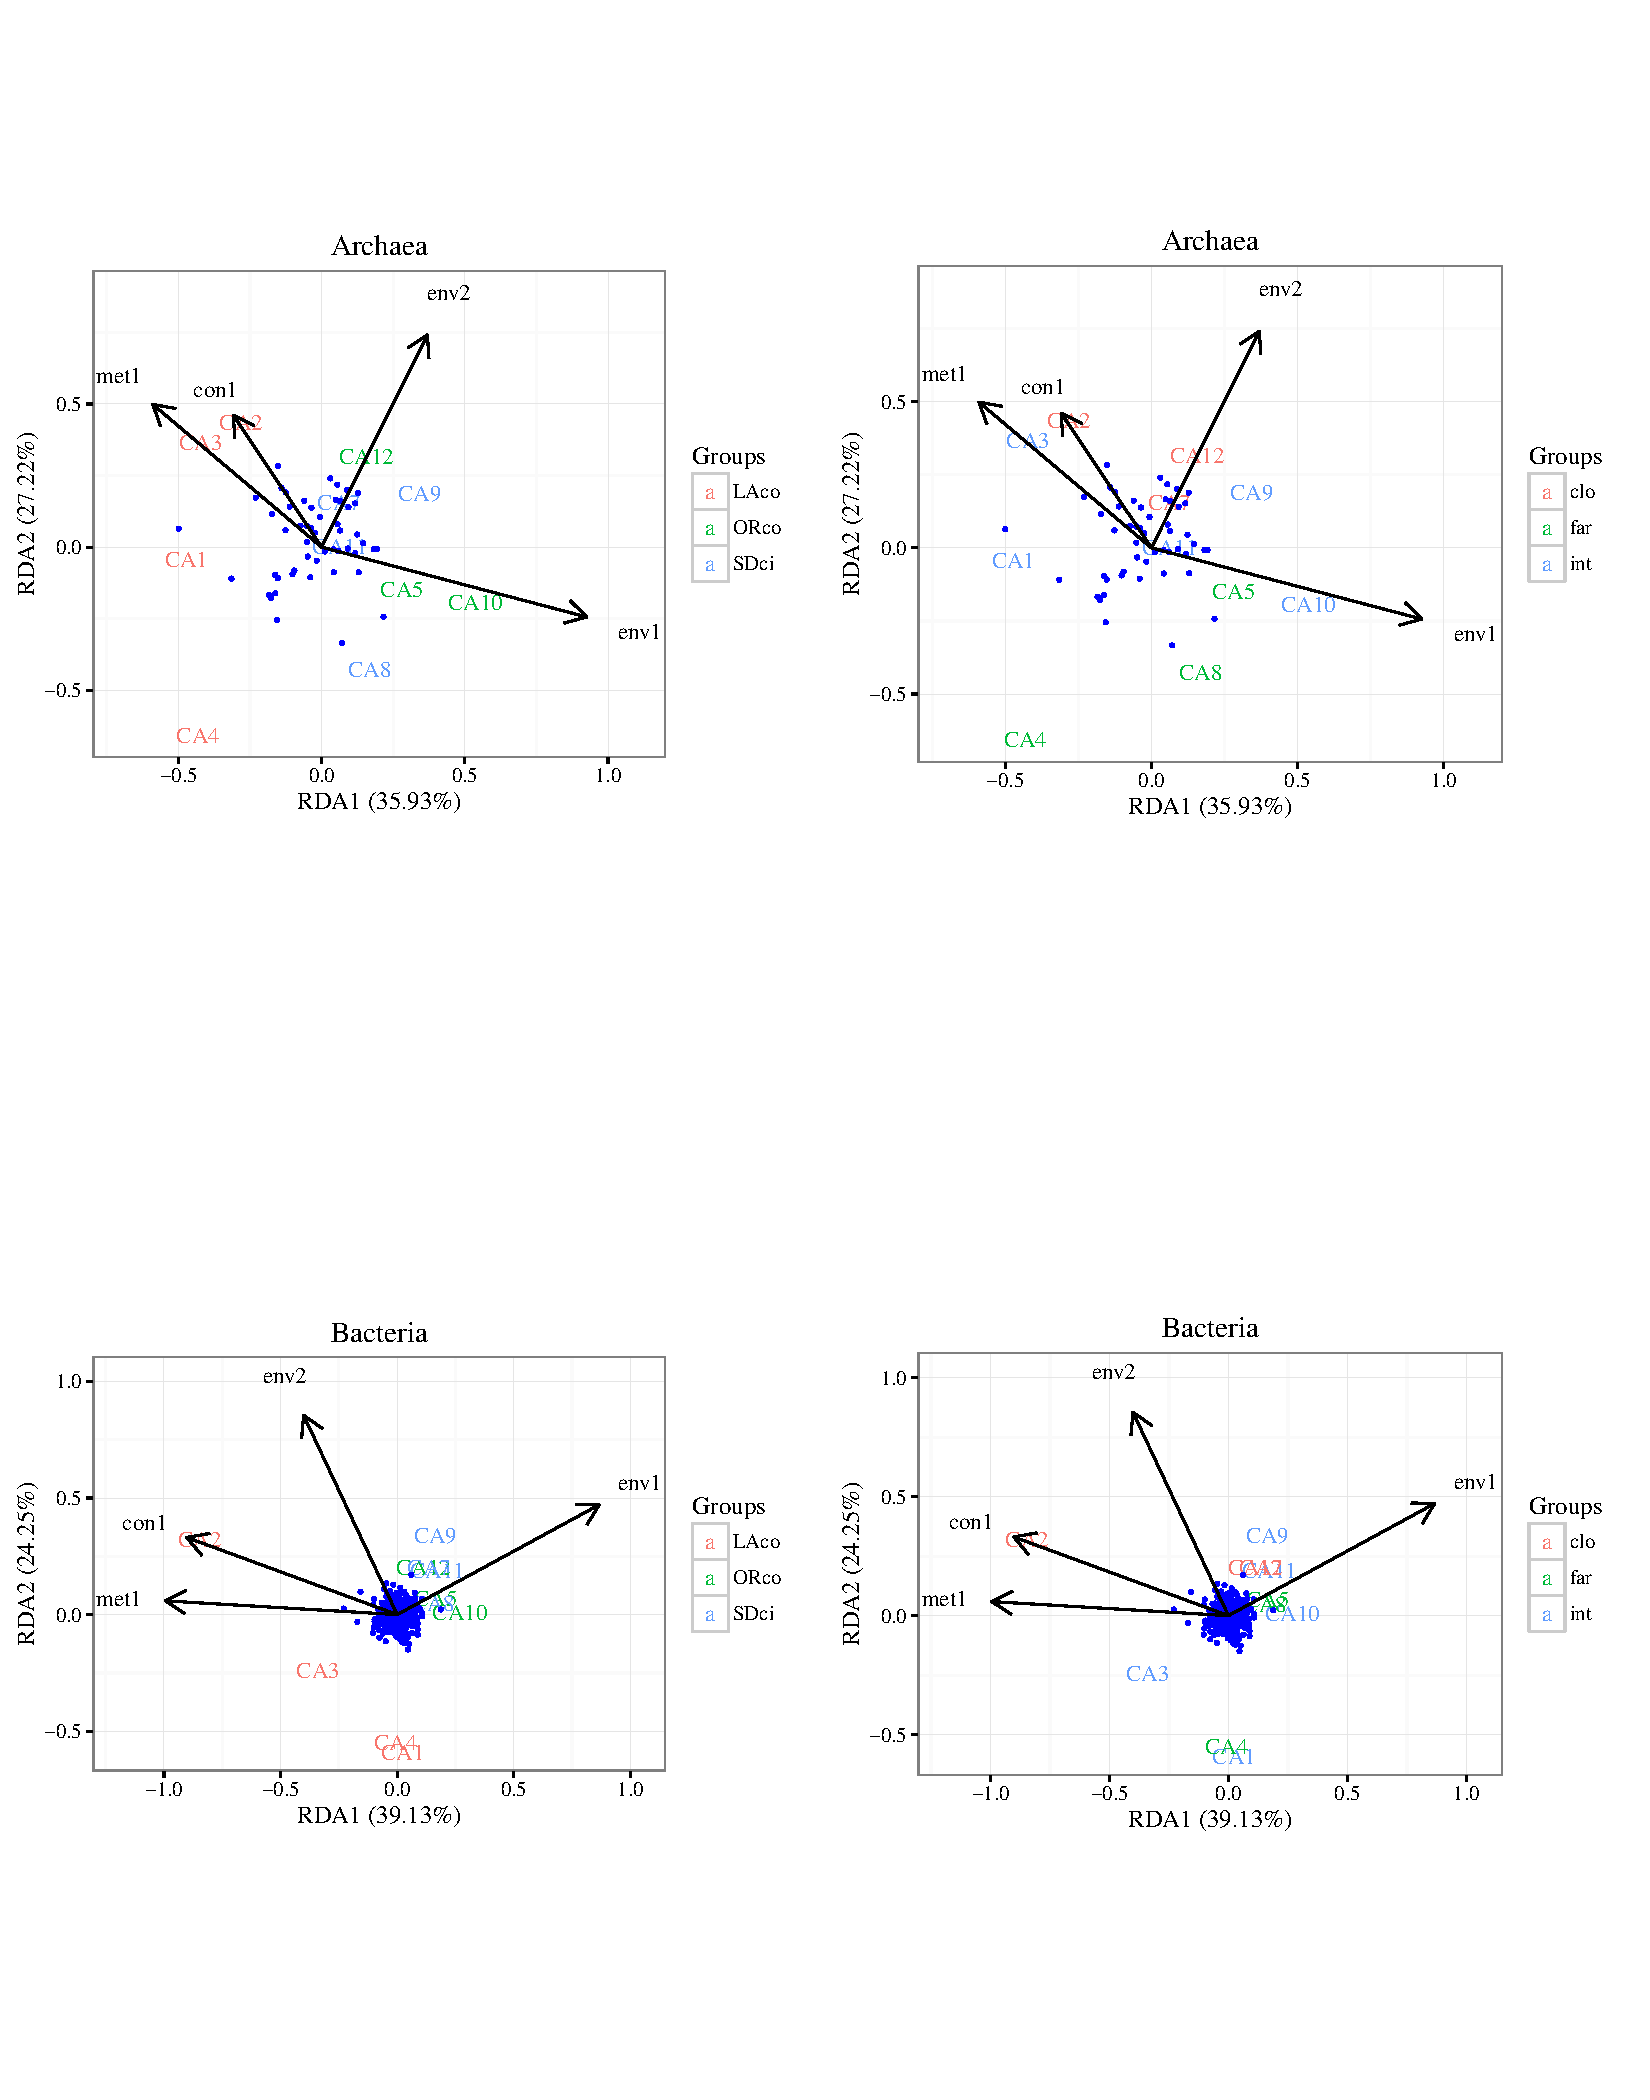
\includegraphics[width=\textwidth]{figs/unnamed-chunk-6-1} 

}

\caption[Constrained ordination analyses (RDA) of species level data in relation to principal component axes that describe contaminants, environmental, and metals data]{Constrained ordination analyses (RDA) of species level data in relation to principal component axes that describe contaminants, environmental, and metals data.  Separate analyses for archaea and bacteria are shown, with site codes grouped by municipality and distance from pipe.}\label{fig:unnamed-chunk-6}
\end{figure}


\end{knitrout}

\begin{knitrout}
\definecolor{shadecolor}{rgb}{0.969, 0.969, 0.969}\color{fgcolor}\begin{figure}[!ht]

{\centering 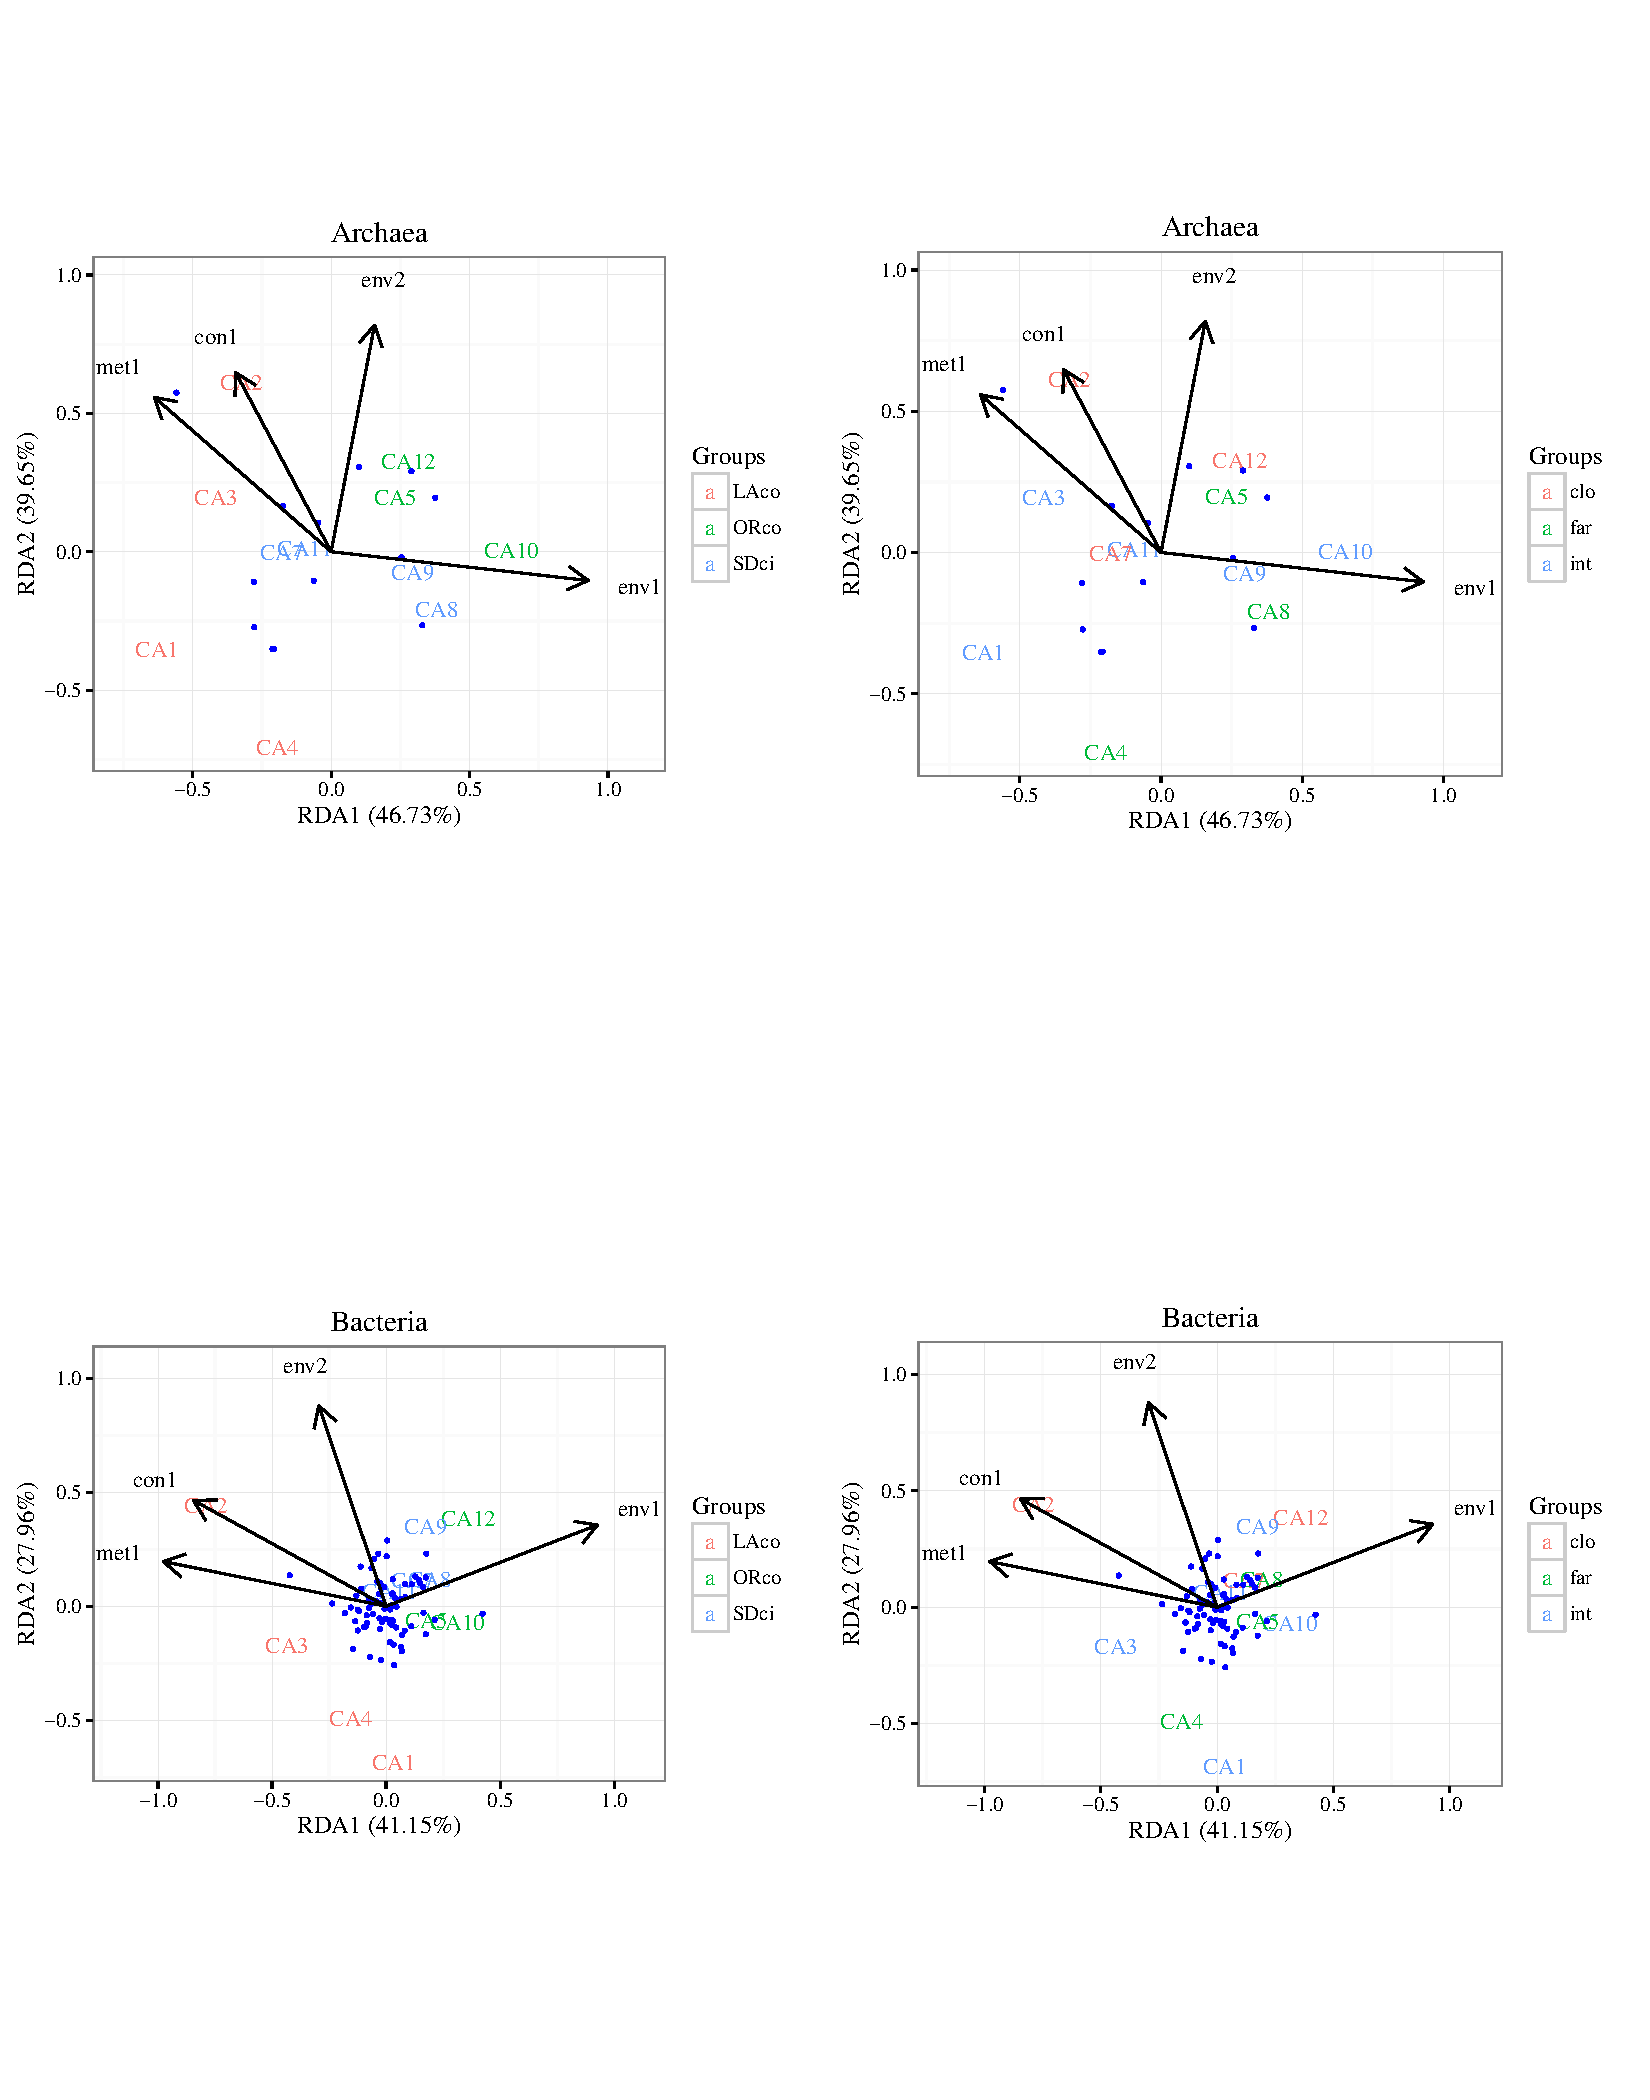
\includegraphics[width=\textwidth]{figs/unnamed-chunk-7-1} 

}

\caption[Constrained ordination analyses (RDA) of orders in relation to principal component axes that describe contaminants, environmental, and metals data]{Constrained ordination analyses (RDA) of orders in relation to principal component axes that describe contaminants, environmental, and metals data.  Separate analyses for archaea and bacteria are shown, with site codes grouped by municipality and distance from pipe.}\label{fig:unnamed-chunk-7}
\end{figure}


\end{knitrout}
\clearpage

\subsubsection{Analyses by municipality}

The above analyses were repeated separately for each municipality. 

\begin{knitrout}
\definecolor{shadecolor}{rgb}{0.969, 0.969, 0.969}\color{fgcolor}\begin{figure}[!ht]

{\centering 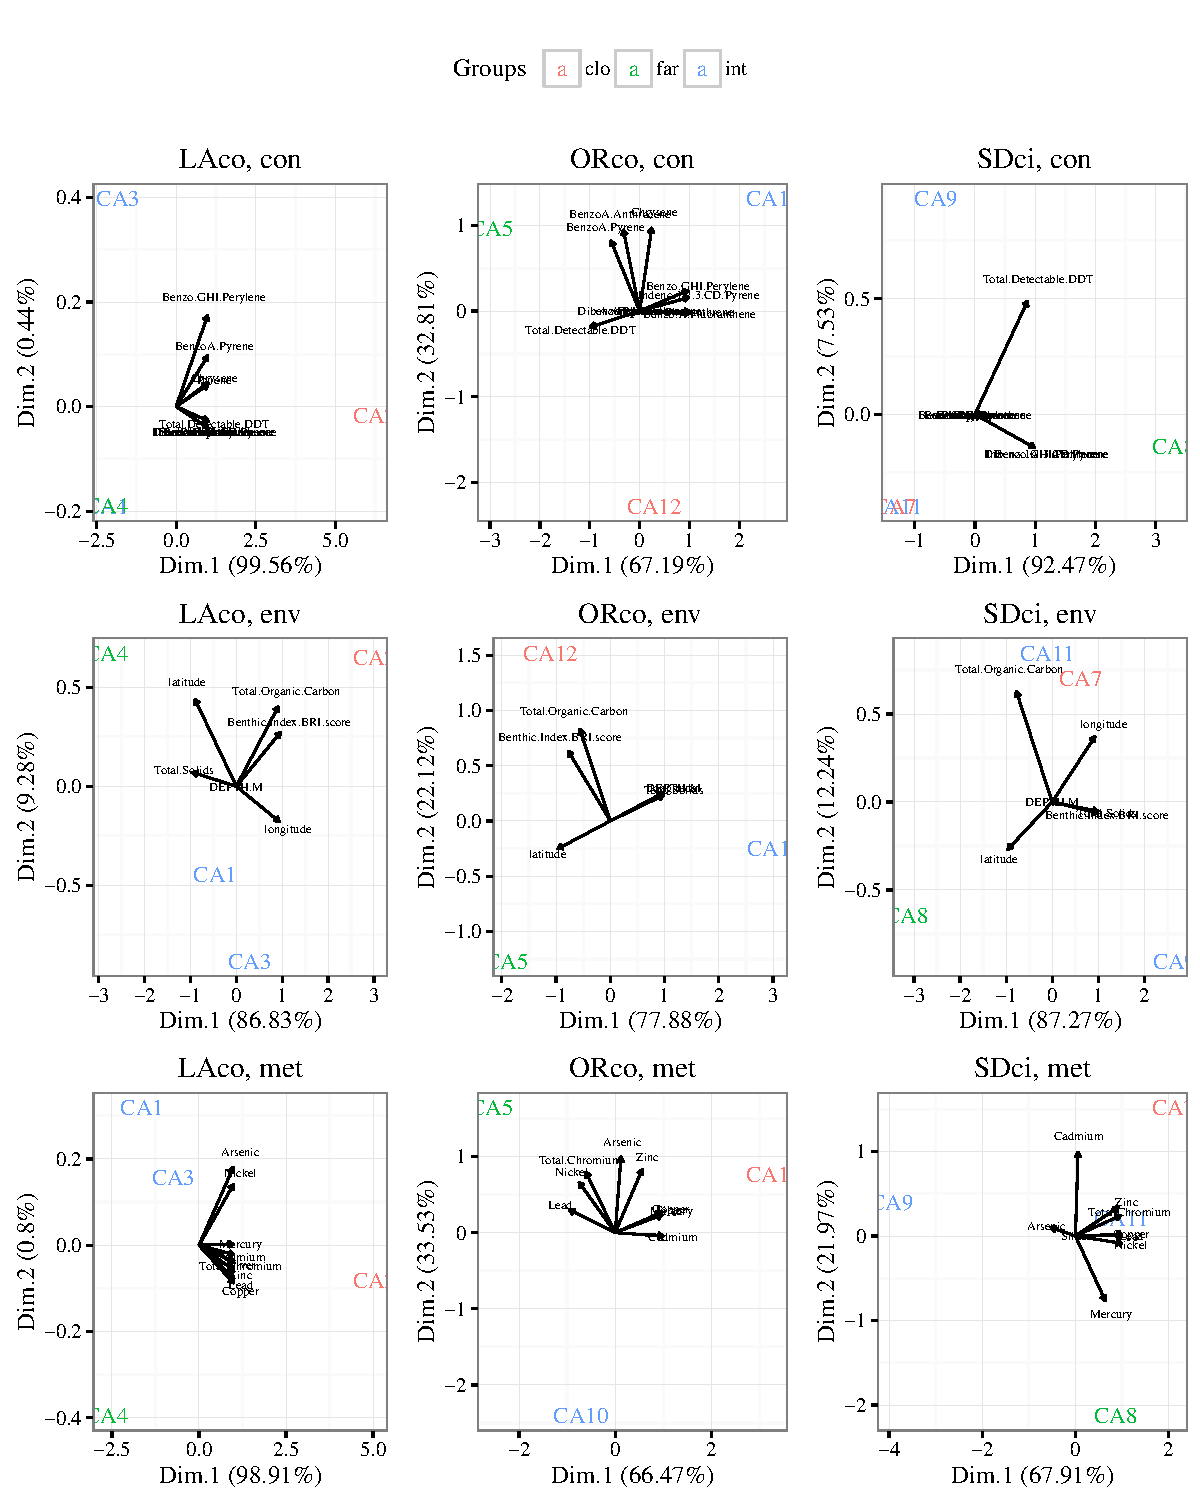
\includegraphics[width=\textwidth]{figs/unnamed-chunk-8-1} 

}

\caption[Principal component axes for contaminants, environmental, and metals, grouped by distance from pipe and separate analyses for each wastewater treatment plant]{Principal component axes for contaminants, environmental, and metals, grouped by distance from pipe and separate analyses for each wastewater treatment plant.}\label{fig:unnamed-chunk-8}
\end{figure}


\end{knitrout}

\begin{knitrout}
\definecolor{shadecolor}{rgb}{0.969, 0.969, 0.969}\color{fgcolor}\begin{figure}[!ht]

{\centering 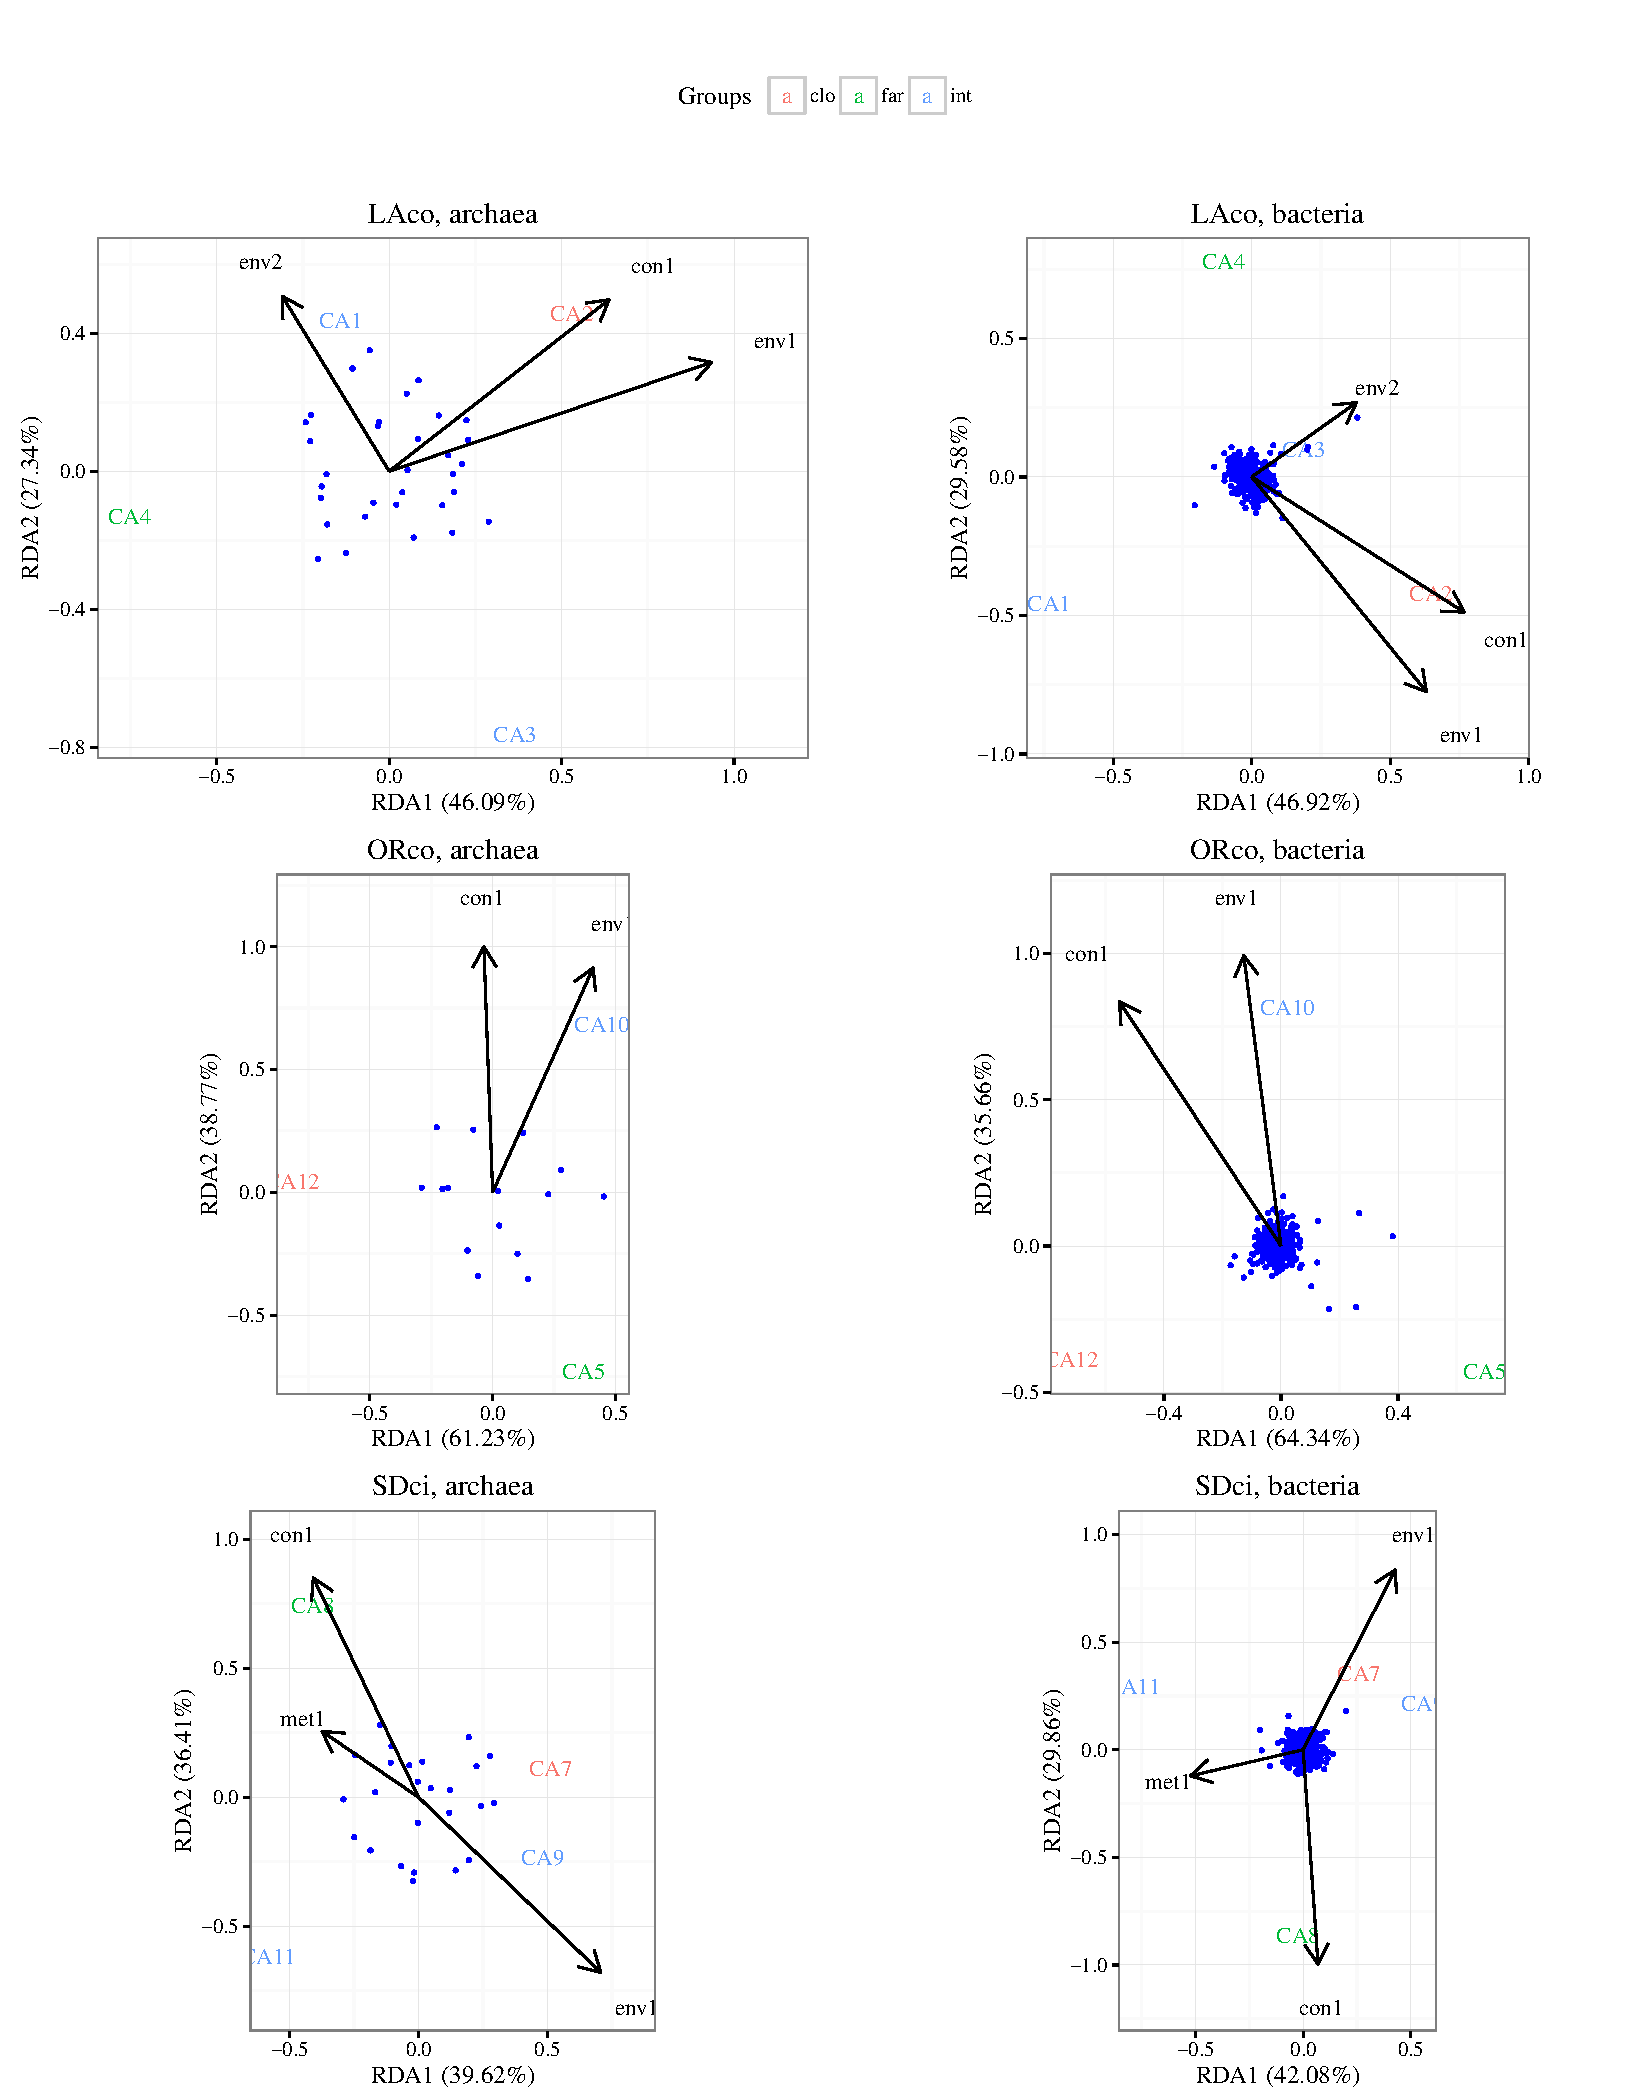
\includegraphics[width=\textwidth]{figs/unnamed-chunk-9-1} 

}

\caption[Constrained ordination analyses (RDA) of species level data in relation to principal component axes that describe contaminants, environmental, and metals data]{Constrained ordination analyses (RDA) of species level data in relation to principal component axes that describe contaminants, environmental, and metals data.  Separate analyses for each municipality and taxonomic groupings of archaea and bacteria are shown.  Site colors indicate approximate distance from pipe.}\label{fig:unnamed-chunk-9}
\end{figure}


\end{knitrout}

\clearpage





\section{Diversity and distance from pipe}

Diversity measures were evaluated in relation to euclidean distance from the end of a WWTP outflow pipe.  Sites at each municipality that were closest to each pipe were assumed to be zero distance.  The distances of all other sites in relation to the closest pipe were measured as euclidean straight-line distance.
\begin{knitrout}
\definecolor{shadecolor}{rgb}{0.969, 0.969, 0.969}\color{fgcolor}\begin{figure}[!ht]

{\centering 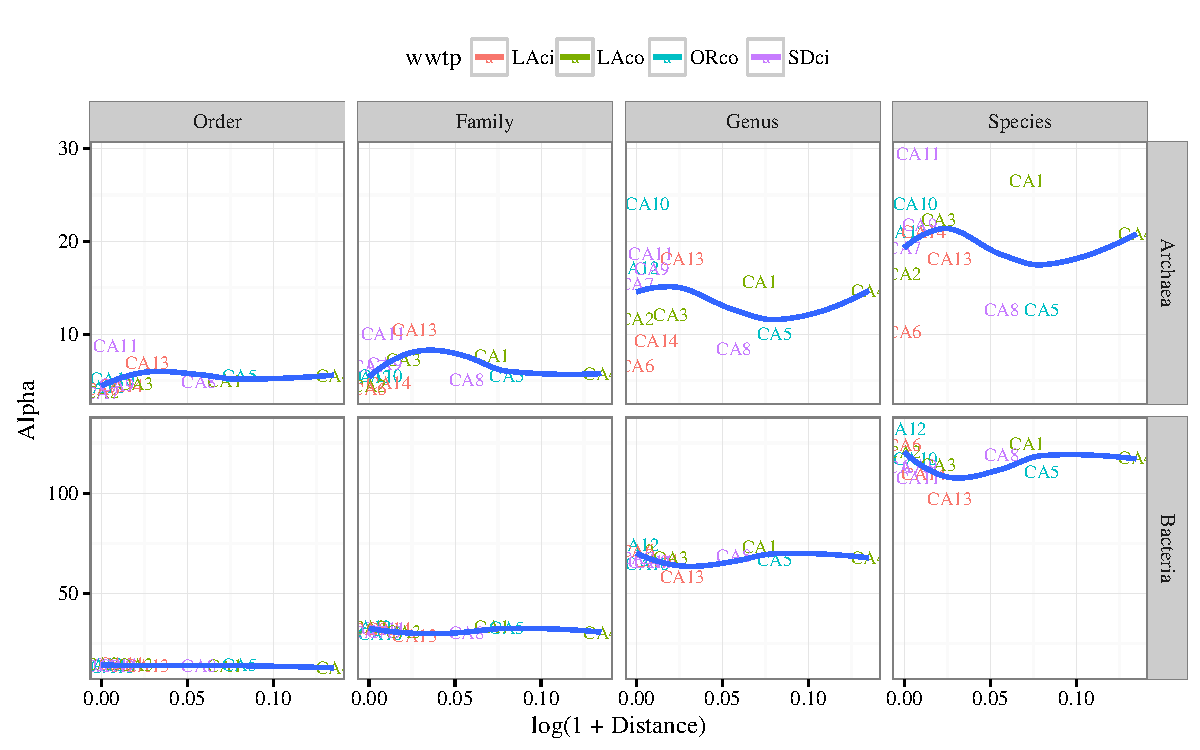
\includegraphics[width=\maxwidth]{figs/alphdist-1} 

}

\caption[Alpha diversity by taxonomic groupings as a function of distance from an outflow pipe at each location]{Alpha diversity by taxonomic groupings as a function of distance from an outflow pipe at each location.  Lines are locally estimated polynomial smooths.}\label{fig:alphdist}
\end{figure}


\end{knitrout}

\section{Interpretation}

Results can be interpreted by considering differences in site groupings potentially related to municipality, distance from pipe, taxonomic resolution, and domain partitions.  Alpha (within a location) and beta diversity (between locations) should also be considered based on these groupings.  Metadata at each site were insufficient to describe community composition.   

Effect of taxonomic resolution:
\begin{itemize}
\item Greater distinction between sites, municipalities, and diversity was achieved with higher taxonomic resolution.
\item Differences between archaea and bacteria were observed, with archae community showing greater distinction getween sites and municipalities, although bacteria diversity was larger
\end{itemize}

Differences between municipalities:
\begin{itemize}
\item Municipalities showed stronger groupings in archaea vs bacteria
\item For both archaea and bacteria, Orange County was most distinct
\end{itemize}

Differences relative to outflow:
\begin{itemize}
\item Categorical descriptions of site location relative to pipes (far, intermediate, close) were coarse as groupings were not obvious in either the cluster or ordination analyses, however...
\item Archaea diversity was maximized at a moderate distance from sewage outflow, whereas bacteria diversity was minimized.  This is shown in the diversity tables as well as \cref{fig:alphdist}.
\end{itemize}

Differences between site:
\begin{itemize}
\item By far, the greatest differences in beta diversity was between sites, i.e., community composition varied the most between sites as compared to differences between municipalities or distance from outflows.  
\item Some sites were routinely outliers in the analyses, e.g., CA13 for bacteria
\end{itemize}

Effects of metadata:
\begin{itemize}
\item No conclusions - PCA suggested extreme collinearity in variable categories as well as extreme outliers for some sites.
\item Stepwise variable selection in constrained ordination analyses did not include any parameters, i.e., ordination of community composition was not better explained by constraining with metadata.
\end{itemize}

\end{document}
